%% Setup Document
\documentclass[]{article}
\usepackage[danish]{babel}
\usepackage[utf8]{inputenc}
\usepackage[margin=2.5cm]{geometry}
\renewcommand{\baselinestretch}{1.5}
\usepackage{pdfpages}
%% Setup Section Counters
\setcounter{secnumdepth}{3}
\setcounter{tocdepth}{3}
%% SetUp Figures
\usepackage{graphicx}
\graphicspath{ {Figures/} }
\usepackage{caption}
\usepackage{subcaption}
\usepackage{geometry}
\usepackage{subfiles}
%% Update Enumerate to make Use Cases possible 
\usepackage{enumerate}
\usepackage{enumitem}
%% Enable figure wrapedin text
\usepackage{wrapfig}
%% Change Subsubsection spacing
\usepackage{titlesec}
\titlespacing{\subsubsection}{0pt}{0.4\baselineskip}{0pt}
%% Unknow
\usepackage{amsmath}
\usepackage{gensymb}
\usepackage{appendix}
\usepackage{float}
\usepackage{textcomp}
\usepackage{lastpage}
\usepackage[T1]{fontenc}
\usepackage{lmodern}
\usepackage{cite}
%
%
%%% Setup frontpage
%\newcommand*{\titleGP}{\begingroup 
%	\renewcommand{\baselinestretch}{1} 
%	\begin{picture}(0, 0) (-390,31)
%	\includegraphics[width=0.12\textwidth]{logo1.png}
%	\end{picture}
%
%	\centering 
%	\vspace*{\baselineskip} 
%	
%	\rule{\textwidth}{1.6pt}\vspace*{-\baselineskip}\vspace*{2pt} % Thick horizontal line
%	\rule{\textwidth}{0.4pt}\\[\baselineskip] % Thin horizontal line
%	
%	{\LARGE Eksamen\\  [0.3\baselineskip]
%		 Holdnummer C6} \\[0.2\baselineskip] % Title
%		 %De sejeste mennesker : Caféen?}\\[0.2\baselineskip] % Title
%	
%	\rule{\textwidth}{0.4pt}\vspace*{-\baselineskip}\vspace{3.2pt} % Thin horizontal line
%	\rule{\textwidth}{1.6pt}\\[\baselineskip] % Thick horizontal line
%	
%%	\scshape % Small caps
%%	Sidste øjekast på applikationen \\
%	
%	
%%	\vspace*{2\baselineskip} % Whitespace between location/year and editors
%	
%	af \\[\baselineskip]
%    {\Large  Camilla Ejsing (smb912@alumni.ku.dk) \\    \par} % Editor list
%%	{\Large  Camilla Ejsing \\ Mohammed Sami Elnono \\ Nicolai Manique \& \\ Søren L. Nissen    \par} % Editor list
%    {Instruktorer: Alexander Winther Uldall \& \\ (Sven Uhrenholdt Frenzel) \par }
%    {GitHub-arkiv: https://github.com/cejsing/Softwareudvikling \par}
%
%%    {Gammelt GitHub-arkiv: https://github.com/samielnono/Project-Cafeen \\
%%    Nyt GitHub-arkiv: https://github.com/SNissen/ProjectCafeenC6 \par}
%	{\itshape Datalogi : Softwareudvikling \par} % Editor affiliation
%	
%	\vfill % Whitespace between editor names and publisher logo
%%	\includegraphics[height=0.4\textheight]{FrontPage.jpg}
%	\vfill
%	{\scshape 2016} \\[0.3\baselineskip] % Year published
%	{\large }\par % Publisher
%	
%\endgroup}
%
\usepackage{pdfpages}
\usepackage{listings}
\lstset{literate=%
{æ}{{\ae}}1
{å}{{\aa}}1
{ø}{{\o}}1
{Æ}{{\AE}}1
{Å}{{\AA}}1
{Ø}{{\O}}1,
basicstyle=\small\sffamily,
escapechar=\&
}
\lstset{language=Python}
\usepackage{color}
\definecolor{bluemail}{rgb}{0.13,0.13,1}
\definecolor{greydate}{rgb}{0.43,0.5,0.5}
\definecolor{purple}{rgb}{0.54,0.17,0.89}


\lstdefinelanguage{Gmail}
{   sensitive=false,
    morecomment=[l][\color{purple}]{>},
    morecomment=[l][\color{greydate}]{Dato},
    }
    
    

\begin{document}
    \thispagestyle{empty}


\includepdf[fitpaper,pages={-}]{forside.pdf}
    \newpage
    
\cleardoublepage
\pagenumbering{gobble}
\tableofcontents
\listoffigures
\listoftables \vspace*{2cm}

\fbox{
\begin{minipage}{\textwidth}
\vspace*{0.3cm}
Denne rapport er baseret på en tidligere rapport, som blev skrevet i samarbejde med gruppemedlemmerne Nicolai Manique (jpm235@alumni.ku.dk) og Søren L. Nissen (rhc148@alumni.ku.dk) (tidligere gruppe C6) og kan ses som et forsøg på forbedring af denne. Nogle af elementerne er derfor meget ens eller identiske. Den tilhørende kode er ligeledes udarbejdet i samarbejde med ovenstående. Figurerne \ref{fig:fileStrk}, \ref{fig:database} og \ref{fig:Change} er ikke ændret fra den tidligere rapport.
\vspace*{0.3cm}
\end{minipage}} \vspace*{0.3cm}

\cleardoublepage

\newpage
\pagenumbering{arabic}

\section{Projektbeskrivelse} \label{Projektbeskrivelse}
% En kort beskrivelse af jeres applikation og dens anvendelse. Væsentlige tolkninger af opgaveteksten, hvor I fandt den tvetydig, og afgrænsninger I har valgt at foretage skal beskrives og begrundes.
Vi blev stillet opgaven at lave et system, der kan lette opgaven for de ansvarlige nøglebærere på studiebaren Caféen?, at lave optællinger ved åbning og lukning af baren. Det nuværende system betegnes som svært at bruge for nøglebærere, der ikke har en bachelorgrad i datalogi. Systemet sørger for, at man nemt kan finde dagens omsætning, som beregnes udelukkende ud fra optælling af varer. Dette afsnit indeholder en afklaring af den stillede opgave, hvor det beskrives, hvordan de stillede krav tolkes og hvordan vi har afgrænset problemet.

\subsection{Beskrivelse af Caféen? - nyt lageroptællingssystem}
Vores løsning på det stillede problem var at kreere et nyt lageroptællingssystem, som skal være let at tilgå for alle nøglebærere uanset uddannelse. Systemet indeholder oversigter over eksisterende varer, varegrupper og begivenheder med mulighed for at rette oplysninger, slette og oprette nye af ovenstående. Systemet indeholder også en historik, så der kan ses rettelser, sletninger og oprettelser. Systemet indeholder ydermere muligheden for at modtage varer og naturligvis åbning og lukning af Caféen?. \\
Det er vigtigt, at de indtastede oplysninger og antal af eksempelvis varer er korrekte, da der ellers vil forekomme fejl i beregning af dagens omsætning. \\
For en dybere beskrivelse af systemet, funktionalitet og design, se afsnit \ref{Krav} og \ref{Design}. \\ \\
Det har i projektbeskrivelsen været lidt tvetydigt, hvorvidt det var ønsket, at alle varer i samme varegruppe skulle have samme pris, eller om dette var en procedure man havde nu, men ønskede at ændre. Da vi har haft fokus på at vores program skal være fleksibelt, har vi valgt at hver enkelt vare har sin egen pris, men der er mulighed for at tilføje prisændringer for hele varegrupper. En specifik problemstilling vi har haft store problemer med at håndtere har været håndteringen af sprut. Det har fra Cafeén?s side været udtrykt, at man ønskede at opgøre sprut i vægt, men det har været svært at finde ud af, hvordan de ønskede denne problemstilling håndteret. Se \ref{Sprut} for nærmere beskrivelse af løsningen på denne problemstilling.

\subsection{Afgrænsninger}
Caféen? er en studiebar og der er derfor tale om et omfangsrigt projekt og system, da systemet skal kunne behandle både ordinære begivenheder såsom en almindelig fredags-bar, men også skal kunne behandle begivenheder såsom ÅDH (åbner for dovne hunde), udlejninger, rabatter til bartendere og nøglebærere og eventuelle forhindringer og undtagelser, man kunne støde ind i som nøglebærer i løbet af en vagt. Vi har derfor skelnet mellem \textit{must-haves} og \textit{nice-to-haves} med fokus på \textit{must-haves}. \\ \\
%
%
%Sammen med min gruppe udviklede jeg et nyt lageroptællingssystem til Caféen?. \\
%Vi lagde vægt på simplicitet i backenden, da der i beskrivelsen af opgaven blev lagt vægt på at koden skulle være simpel og let at ændre. \\
%Applikationen er kodet sådan, at backenden indeholder funktioner, der kan håndtere forskellige problemer, og frontenden eksekverer så disse funktioner på fornuftig vis. Dette gør det nemt for en anden programmør at sætte sig ind i hvordan koden fungere, og ønsker man at tilføje en funktion kan man blot udbygge den nuværende kode. Dette gør programmet yderst fleksibelt og nemt at gå til. Ud over dette var der også et ønske om at kunne håndtere forskellige varegrupper og begivenheder med forskellige priser. Dette var noget af det første vi kastede os over, og det har været vores fokus at få disse tre ting til at fungere. Ud over dette har historikken været noget der i opgavebeskrivelsen var lagt vægt på historikken. At man kunne gå tilbage i tiden og se ændringer, eller rettere, ændringer skulle ikke gælde bagud. Vi har valgt at lægge fokus på at kunne følge ændringernes gang. Dette kan der læses mere om koden afsnittet "Design". Alt i alt kan man opsummere vores fokus punkter til: 
%\begin{enumerate}
%	\item \textbf{Simpel backend} \\ Skal være til at overskue hvor ting ligger.
%	\item \textbf{Nemt at ændre} \\ Skal ikke være et låst program, det skal kunne viderusvikles.
%	\item \textbf{Brugbart udgangspunkt} \\ Vare, varegrupper og begivenheder klar til brug.
%	\item \textbf{Simpel håndtering af historik} \\ Skal ikke forstyrre funktionen af resten af programmet, og skal være nemt at tilgå. 
%\end{enumerate}

\indent For første release medio juni forventedes det, at brugeren kunne tilføje en vare til systemet med valgt varegruppe og pris. Det forventedes at brugeren kunne åbne og lukke en vagt med optællinger som korrekt ville videregå til databasen over varer. Det forventedes derudover, at en yderligere udvikling nemt kunne understøtte yderligere funktionaliteter i henhold til brugerens oplyste behov. \\
\indent I henhold til brugerens ønsker vil fokus primært være udvikling af backend/database. Databasen vil blive implementeret med tabeller og relationer i forhold til udviklet design og backend vil blive udviklet med fokus på at manipulere databasen på en måde, der passer til kundens krav.

\pagebreak[3]

\section{Krav} \label{Krav}
Kravene til en applikation kan inddeles i kvalitative krav og funktionelle krav, hvor kvalitative krav eksempelvis kan være brugervenlighed og funktionelle krav kan beskrives som en række use cases.
Der blev ligeledes sat to tekniske krav til projektet, hvor det kræves at projektet skrives i enten programmeringssproget C\# eller Python, og at programmet skal være brugbart for Caféen?.

\subsection{Kvalitative krav}
For at kunne opskrive de kvalitative krav, har vi gennemgået projektbeskrivelsen og taget noter til et møde fra opstarten af projektet, hvor kunderepræsentanten Jenny klargjorde behovene for et nyt lageroptællingssystem. Dette gjorde vi for at klargøre de givne krav og undersøge, hvordan vi kan få vores program til at imødekomme disse krav.
\begin{itemize}
 	\item \textbf{Simplicitet og neutralitet (og det skal ikke indeholde "fancy features")} Systemet skal være nemt at bruge og det skal være neutralt. Dette opnås ved at fokusere på et system, hvor der let kan oprettes, rettes og slettes varer.
 	\item \textbf{Det skal være webbaseret} Vi vælger at opsætte en hjemmeside, hvorfra man på simpel vis kan foretage optælling af baren.
 	\item \textbf{Let anvendeligt} Det skal være nemt for alle brugere at benytte systemet - også for ikke-dataloger. Derfor har vi planlagt at brugerfladen skal være simpel, hvilket også kommer til udtryk i punktet om simplicitet og neutralitet.
 	\item \textbf{Historik} Det skal være muligt at se historikken for vareændringer, ændringer i begivenheder og tidligere optællinger.
 	\item \textbf{Anvendeligt for flere brugere} Det skal være muligt at flere brugere tilgår systemet samtidig, uden at der kommer fejl i de indtastede data. Dette løses som del af historikken, hvor der som fremtidig use case er planlagt at muliggøre login fra brugere samt koble brugerID sammen med historikken.
\end{itemize}

\subsection{Funktionelle krav}
Vi har lavet to use cases på fuld form, som beskrevet i \textbf{Cockburn} i afsnit \ref{UseCase1} og \ref{UseCase2}, og resten er lavet på kort form. Disse use cases tjener som de funktionelle krav, vores system skal kunne. \\ \\
I den agile proces udarbejdes use cases først på kort form. Ud fra disse use cases vælger kunden de use cases, der ønskes implementeret først. Disse use cases bliver undersøgt nærmere og sættes på fuld form, hvor den forventede tid brugt på den givne use case anslås. Man skal forsøge at planlægge på en sådan måde, at det er muligt at implementere de planlagte use cases i løbet af en enkelt iteration, som i vores tilfælde har været en måned. Det er på denne måde muligt at lave et del-release efter hver iteration, hvorved samarbejdet med kunden opretholdes og det er muligt løbende at sikre, at de kvalitative krav er overholdt. \\
De use cases, der er skrevet på kort form kan ses i afsnit \ref{UseCasesShort}.
\subsubsection{Use case - Tilføj vare} \label{UseCase1}
\fbox{
\begin{minipage}{\linewidth}
\vspace*{0.3cm}
\textbf{Primær aktør} Bruger (Nøglebærer) \\
\textbf{Mål} At oprette en ny vare til systemet
	\begin{enumerate}
	\setlength{\itemsep}{-3pt}
		\item Nøglebærer klikker på "Ny vare"
		\item Info om den nye vare udfyldes (navn, standardpris og varegruppe)
		\item Nøglebærer klikker "Gem"
		\item Varen er nu oprettet og indskrives i databasen for de relevante tabeller
	\end{enumerate}
\textbf{Udvidelser til den nominelle case}: \\
3a1 Der mangler info om varen \\
3a2 Fejlmeddelelse vises med info om manglende felter \\
3a3 Nøglebærer udfylder de manglende informationer \\
3b1 Varen eksisterer allerede \\
3b2 Fejlmeddelelses vises med info om at navnet er i brug \\
3b3 Nøglebærer udfylder manglende informationer 
\vspace*{0.3cm}
\end{minipage}} \vspace*{0.3cm}
\subsubsection{Use case - Ændre priser på en vare} \label{UseCase2}
\fbox{
\begin{minipage}{\linewidth}
\vspace*{0.3cm}
\textbf{Primær aktør} Bruger (Nøglebærer) \\
\textbf{Mål} At ændre information for en begivenhed
	\begin{enumerate}
	\setlength{\itemsep}{-3pt}
		\item Nøglebærer klikker på ønsket begivenhed
		\item Nye informationer indtastes
		\item Nøglebærer klikker "Gem"
		\item De nye informationer gemmes og indskrives i databasen for de relevante tabeller
	\end{enumerate}
\textbf{Udvidelser til den nominelle case}: \\
3a1 Det nye navn eksisterer allerede \\
3a2 Fejlmeddelse vises \\
3a3 Nøglebærer udfylder de manglende informationer \\
3b1 Begivenheden slettes
\vspace*{0.3cm}
\end{minipage}} \vspace*{0.3cm}
\subsubsection{Implementerede use cases} \label{UseCasesShort}
\noindent På de 5 måneder, vi havde til rådighed, kunne vi nå i alt 5 iterationer. I den første iteration brugte vi tiden på at udforske det framework, vi skulle bruge og planlægge, hvad vi ønskede at implementere. \\
I iteration 2, 3, 4 og 5 implementerede vi løbende use cases og fandt løbende flere use cases. Visse use cases nåede vi ikke at implementere, hvoraf vi havde vurderet nogle af dem som \textit{nice-to-haves}.
\subsubsection*{Use cases til 2. iteration}
\fbox{
\begin{minipage}{\linewidth}
\vspace*{0.3cm}
	\begin{itemize}
	\setlength{\itemsep}{-3pt}
		\item  \textbf{Tilføj vare til systemet} Det vælges at tilføje en ny vare. Nøglebærer skal notere navn, standardpris (og varegruppe).
		\item \textbf{Tilføj varegruppe} Det vælges at tilføje en ny varegruppe. Nøglebærer skal notere navn og der kan tilføjes en beskrivelse, hvis ønsket.
	\end{itemize}
\end{minipage}} \vspace*{0.5cm}
\subsubsection*{Use cases til 3. iteration}
\fbox{
\begin{minipage}{\linewidth}
\vspace*{0.3cm}
	\begin{itemize}
	\setlength{\itemsep}{-3pt}
		\item \textbf{Tilføj vare til varegruppe} Vare og varegruppe skal eksistere. Brugeren kan ændre varens tilhørsgruppe ved at ændre information om den givne vare.
		\item \textbf{Ændre priser på en vare fremadrettet} Nøglebærer vælger vare, der skal ændres pris for. Den nye standardpris sættes.
		\item \textbf{Ændre information om vare} Nøglebærer vælger vare, der skal ændres pris for. Den nye information noteres.
	\end{itemize}
\vspace*{0.3cm}
\end{minipage}} \vspace*{0.5cm}
\subsubsection*{Use cases til 4. iteration}
\fbox{
\begin{minipage}{\linewidth}
\vspace*{0.3cm}
		\begin{itemize}
		\setlength{\itemsep}{-3pt}
			\item  \textbf{Opret begivenhed med specificerede priser} Der oprettes en ny begivenhed, hvor der noteres navn og prisændringer.
			\item  \textbf{Åben med begivenhedsspecificerede priser} Særlige begivenheder kan vælges ved åbning af baren. Her indtastes antal varer i bar og på lager.
			\item  \textbf{Slet vare i systemet} Nøglebærer vælger vare, der ønskes slettet. Dette noteres i historikken.
			\item  \textbf{Optælling på seddel indtastes senere} Denne indtastning kan foregå som en almindelig eller hvilken som helst anden begivenhed, hvor der både skal åbnes og lukkes.
		\end{itemize}
\vspace*{0.3cm}
\end{minipage}} \vspace*{0.5cm}
\subsubsection*{Use cases til 5. iteration}
\fbox{
\begin{minipage}{\linewidth}
\vspace*{0.3cm}
	\begin{itemize}
	\setlength{\itemsep}{-3pt}
		\item  \textbf{Lager optælles ved åbning} Nøglebæreren vælger den ønskede begivenhed, der skal åbnes, hvori der er en liste med varer, hvor tomme felter skal udfyldes med antal i hhv. bar og på lager.
		\item \textbf{Lager optælles ved lukning} Nøglebæreren vælger at lukke Caféen?, hvor der skal udfyldes antal varer i hhv. bar og på lager.
		\item  \textbf{Håndtering af vægt af sprut} Ved oprettelse af varen "sprut"\, indtastes en startvægt. Ved åbning og lukning af Caféen? registreres åbningsvægt og vægt ved lukning. Ud fra dette beregnes salg.
		\item  \textbf{Foretag varemodtagelse} Baren skal være lukket, så der ikke opstår fejl ved senere optælling. Herfra kan vælges at ændre informationer for eksisterende varer (såsom antal), og oprettes nye varer.
		\item  \textbf{Ændre prisen for varegruppe} Den ønskede varegruppe vælges, og der kan ændres både pris og information for varegruppen. 
		\item \textbf{Tilføj kommentar til optælling} Nøglebærer kan skrive en kommentar til optælling (både åbning og lukning), som kan ses i historikken.
		\item \textbf{Vis komplet vareliste} Den komplette vareliste vises på siden.
	\end{itemize}
\vspace*{0.3cm}
\end{minipage}} \vspace*{0.5cm}

\subsubsection{Fremtidige use cases}
\noindent Der er nogle use cases, vi ikke fik implementeret i løbet af de 5 iterationer. Disse fleste af disse use cases blev betegnet som \textit{nice-to-haves}, og det gav bedst mening for os, at implementere dem sent i processen. \\
Den use case, der er vigtigst at implementere fremtidigt er  \\
\fbox{
\begin{minipage}{\linewidth}
\vspace*{0.3cm}
\textbf{Identificér optæller} Muliggør login, identificér nøglebærer og notér i historik.
\end{minipage}}  \vspace*{0.5cm}

Denne use case påbegyndte vi, men nåede ikke at færdigimplementere. Det er tanken, at nøglebærere skal logge ind for at kunne foretage optælling, og at der er rettighedsforskelle for de enkelte nøglebærere, således at nogle kun kan åbne/lukke baren, mens andre også kan tilføje eller fjerne nøglebærere fra systemet. \\ \\
I det nuværende system har alle adgang. Det kræver altså ikke et særligt brugernavn eller løsen at tilgå og ændre i lagersystemet. \\ \\
Vi har følgende use cases, som kunne være interessante for systemets fremtidige succes:
\subsubsection*{Fremtidige usecases}
\fbox{
\begin{minipage}{\linewidth}
\vspace*{0.3cm}
	\begin{itemize}
	\setlength{\itemsep}{-3pt}
		\item \textbf{Identificér optæller}
		\item \textbf{Flere skal kunne ændre samtidig}
		\item \textbf{Vælg en prisliste (begivenhedtype)}
		\item \textbf{Kasserer vil gerne kunne opholde sidste års indtægter og udgifter i et regnskab}
		\item \textbf{Merge varer}
		\item \textbf{Printe grafer over forskellige salgs-/prisudviklinger}
	\end{itemize}
\end{minipage}}  \vspace*{0.5cm}

\pagebreak[3]

\section{Udviklingsmiljø} \label{Udviklingsmiljo}
% Beskriv jeres udviklingsmiljø, herunder anvendte programmeringsmiljø, opsætning af projektet i GitHub, plan for versionsstyring, mv. Forklar hvordan filer i projektet er struktureret. Forklar endvidere hvordan jeres applikation bygges og afvikles.
% Dette afsnit skal kunne læses af nye udviklere som vejledning i at sætte et udviklingsmiljø op og påbegynde videreudvikling på projektet.
% I skal endvidere diskutere, hvordan jeres udviklingsmiljø og de værktøjer I har brugt, effektivt understøtter arbejde med programmering, refaktorering, afprøvning og afvikling af applikationen.
Dette afsnit beskriver de tekniske redskaber og værktøjer, vi har brugt til at udvikle applikationen. Det er tænkt at give en grundlæggende introduktion til programmeringssproget, Python, det brugte framework, Django og vores brug af GitHub. Dette afsnit er en god forudsætning for at kunne forstå de følgende afsnit i denne rapport, navnligt afsnit \ref{Design} om designet af applikationen. 
% gennemgå vores udviklingsmiljø. Vi vil gennemgå opsætning af vores undeliggende teknologi, Python - Django \& SQLite - samt valget af værktøjer, PyCharm, Kate og GIT.

\subsection{Underliggende teknologi}
De underliggende teknologier, benyttet i projektet, har været Django som importeret modul til Python. Den benyttede database er SQLite. % , selvom denne var abstraheret væk i Djangos biblioteker.
\subsubsection{GitHub}
\noindent GitHub er et versionsstyringsværktøj til softwareudvikling. Det understøtter udviklingsprocessen ved at have issues, forgreninger og struktur, der tillader flere at arbejde på samme projekt uden at det individuelle arbejde kommer i konflikt med hinanden. \\
Det var et krav, at GitHub skulle benyttes til dette kursus. Hvert gruppemedlem havde en seperat branch til at synkronisere med, og alle kunne derfra merge med master-branchen. \\
Vores use cases blev oprettet som issues på GitHub, så vi kunne holde styr på, hvem der lavede hvad. \\ Dette var ikke uden udfordringer, hvilket bliver diskuteret i afsnit \ref{Diskussion}.
\subsubsection{Python}
\noindent Python blev valgt af gruppen fordi det var et programmeringssprog som alle i gruppen havde et vist kendskab til. Python kan både benyttes som et scripting-sprog og et objektorienteret sprog. \\
Python er et high-level programmeringssprog, som fokuserer på at være rent og letlæseligt. Python er et fortolket sprog, som egner sig godt til webapplikationer. \\
Kendetegnende ved Python er det manglende behov for kompilering og den relativt svage typecheckning. Det manglende behov for kompilering muliggør, at man hurtigt kan køre en automatiseret test efter en ændring eller teste manuelt efter hver kodet linie. Disse muligheder er blevet benyttet til at raffinere koden flere steder uden at opleve ventetider \cite{martin2006agile,mcconnell2004code}.
\subsubsection{Django}
\noindent Django blev valgt på anbefaling baseret på, at det både indeholder fleksible værktøjer til manipulation af en database og værktøjer til at konstruere hjemmesider med indbyggede sikkerheder mod blandt andet SQL-injections. Da det er et at kravene, at lagersystemet er webbaseret, var det et nemt valg.  \\ \\
Django er et veldokumenteret \cite{DjangoDoc} open-source framework skrevet i Python. Frameworket er udviklet med henblik på, at gøre arbejdet lettere, når man udvikler komplekse apps, der er drevet af databaser. Hele frameworket er skrevet således, at det er baseret på en model-view-controller-arkitektur, hvor den relationelle database er opbygget af datamodeller og Djangos dertilhørende metoder svarer til "Model", Djangos brug af views, som kan bearbejde HTTP-requests med HTML-templates svarer til "View", og den indbyggede url-manager svarer til "Controller". % Desuden har Django andre indbyggede features, herunder login- og brugersystemer med justerbare rettigheder. \\ \\
%Derudover gav førstehåndsindtrykket os et håb om, at vi ikke behøvede at bevæge os meget ud for dokumentationen for at få svar på problemstillinger, man kunne støde på i forbindelse med brug af teknologien. Dette viste sig at få os til at undervurdere bestemte funktioners tidsmæssige omkostninger. \\
%
%\indent I forhold til Djangos indbyggede funktionaliteter er særligt fem moduler blevet benyttet: Models, Forms, Views, URLs og Testscases. Derudover er Djangos templates også blevet benyttet til at generere browsersiderne. \\
\texttt{Models} gjorde det muligt for os at oprette og manipulere med databasen, som var det simple objekt. Inden vi opdagede denne mulighed, havde vi allerede oprettet flere af de fornødne SQL-koder for at opnå den ønskede funktionalitet, men muligheden for at indkapsle disse koder med en større sikkerhed for at undgå fejl var en klar fordel for projektet. Mere komplekse SQL-kommandoer krævede brug af et særligt Q-object fra \texttt{Models}, men dette viste sig ikke at være en større udfordring for projektet. \\ \\
\texttt{Forms} gjorde det muligt at manipulere med \texttt{Models} baseret på input givet at slutbrugeren. Med denne funktionalitet stødte vi ind i en række problemer, hvilket har mindsket vores fulde udbytte af teknologien. Det har bl.a. vist sig, at \texttt{Forms}-klasser ikke er designet til at skulle indgå flere gange på samme side, hvorimod almindelige HTML-forms godt kan skrives ind i en for-løkke. Derudover var det en begrænsning for udviklingen af en frontend, at vi i en stor del af projektet ikke troede, at det var muligt for os, at få \texttt{Forms}-klasser til at kalde vores egne funktioner fra \texttt{Models}, da vi dermed ville miste vores mulighed for at udvikle begrænsninger og oprettelse af historik. \\ \\
\texttt{Views-klasserne} var påvirket af udfordringerne med \texttt{Forms}. Derudover viste de sig mindre intuitive end \texttt{Views}-metoder, hvorfor \texttt{Views} er benyttet i den endelige kode. Muligheden for at kunne tilgå templates og håndtere requests har været en stor hjælp i produktionen af en brugergrænseflade. Brugergrænsefladen bryder med nogle af designprincipperne fra \textbf{Agile} \cite{martin2006agile} og \textbf{Code Complete} \cite{mcconnell2004code}, men i denne del af projektforløbet blev funktionaliteten vurderet til at vægte højere. \\ \\
HTTP-requests bliver håndteret igennem \texttt{urls.py}, hvor de views, der skal linkes til en given url defineres. Filen holder også styr på projektets sider og undersider. Funktionerne i view-filerne bearbejder de indkomne HTTP-requests og eventuelt indtastet data kan hentes og videresendes.
%Djangos \textbf{URLs} håndterede hvilke sider der kunne tilgås og hvilke view-metoder disse sider skulle kalde. \\ \\
%Djangos \textbf{TestCases} gjorde det nemt at udvikle automatiserede tests så snart vi i gruppen havde besluttet os for en konvention for placering af den funktionelle kode. TestCases fungerer ligesom eksempelvis Junit ved at teste asserts og returnere en liste af fejl forbundet med koden. Disse fejl kan være exceptions som den funktionelle kode har kastet eller at ens assertions ikke har givet det korrekte resultat. \\ \\
%Djangos \textbf{templates} gjorde det muligt at fremvise kode fra views og forms gennem en kontekst som blev sendt fra views-metoderne. Der var en del problemer med brugen af denne teknologi, da Djangos templates benytter et hjemmestrikket sprog til at håndtere denne kontekst. En af udfordringerne var at to lister af elementer ikke kunne gennemløbes sideløbende. Man kan med templates hente første element af en liste med \textit{"liste.0"} og få en int baseret på antallet af løkkegennemgange med \textit{forloop.counter0}. Det var dog ikke muligt at hente elementer fra listen ved hjælp af \textit{forloop.counter}, da \textit{liste.forloop.counter0} ikke først ville oversætte løkken, men i stedet ses som en kommando for liste. \\


\subsection{Brug af værktøjer}
Som distribution og versioneringsværktøj har GitHub været benyttet.
I vores første delaflevering lagde vi op til, at der ikke skulle standardiseres om en bestemt IDE til udvikling. Til det efterfølgende møde med instruktorerne blev det krævet at vi alle benyttede PyCharm. Det viste sig dog at PyCharm ikke understøtter skærme med høj opløsning i Linux, hvilket gjorde programmet svært at anvende. Derfor benyttede Nicolai sig af programmet Kate, der er en simpel tekstbehandler med understøttelse af en række af de værktøjer, som bliver anbefalet i \textbf{Code Complete} \cite{mcconnell2004code}. Dog manglede Nicolais IDE \textit{error detection}, \textit{interactive help}, \textit{templates} og \textit{mergetools}. 
% Den sidste af disse værktøjer lå muligvis bag GitHub-problemerne beskrevet i afsnit XXXX .

Søren og Camilla benyttede PyCharm og havde derfor adgang til følgende værktøjer fra PyCharm: \\
\textit{Merge funktion}, som giver et simpelt og nemt overblik når forskellige udgaver skal samles til en. \textit{GIT forbindelse}, som giver nem pull og push håndtering, samt simpel håndtering af forskellige grene af projektet.

\pagebreak[3]

\section{Design} \label{Design}
Dette afsnit beskriver den tekniske udformning og designet af applikationens funktionalitet. Her vil designet blive præsenteret, og vi vil begrunde vores valg af design. Efter at have læst dette afsnit skulle læseren gerne kunne se sammenhængen mellem vores viden om softwaredesign, de stillede krav til applikationen og det endelige resultat. Samtidig tydeliggøres udviklingsmiljøet, som beskrevet i afsnit \ref{Udviklingsmiljo}. \\

\subsection{Filstruktur i applikationen}
Som udgangspunkt til vores design er der brugt Django. Dette giver en struktur, hvor objekter ikke kender til hinanden, medmindre det er strengt nødvendigt. Django har en filstruktur, hvor forskellige objekter skrives i forskellige filer, og det hele administreres af filen \texttt{manage.py} (figur \ref{fig:fileStrk}). Udover disse filer har vi også \texttt{tests.py}, som beskrives nærmere i afsnit \ref{Afprovning}.
% denne fil og dens historie, funktioner og placering på kortet kan der læses mere om i afsnit \ref{Afprovning}.
\begin{figure} [H]
	\centering
	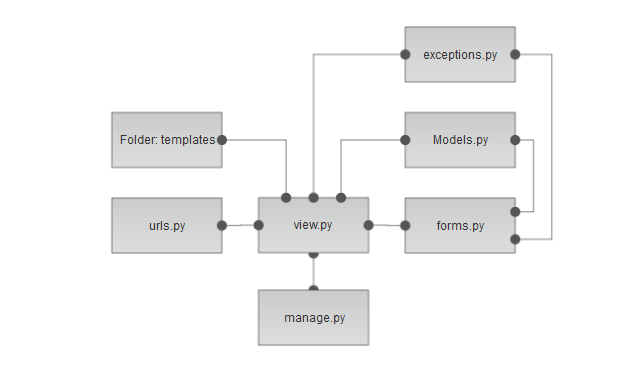
\includegraphics[width = \textwidth]{FileStruct.png}
	\caption[Filstruktur]{Kommunikationen mellem filerne i projektet.}
	\label{fig:fileStrk}
\end{figure}

\noindent Til at komme igang med vores projekt, har vi benyttet os af introduktionen til Django. Denne introduktion tager udgangspunkt i en hjemmeside til at lave meningsmålinger, hvorfor vores program indeholder udtryk som mappen \texttt{polls}. \\
Vi har talt om at fjerne dette, da det kan virke vildledende, men har valgt ikke at gøre det, da der er meget, der henviser til \texttt{polls} i applikationen. \\
Oprettelsen af et Django-projekt gennem introduktionen har medført et stort antal filer, hvor vi i gruppen har været i tvivl om, hvilke der bruges af Django, hvorfor de ikke er slettet.

\subsection{Kodens struktur}
I \texttt{models.py} har vi placeret alle tabeller i databasen - også omtalt som classes eller klasser - og deres tilhørende funktioner. \\
Strukturen af \texttt{models.py} er således, at de forskellige classes kun kender til hinanden, hvis der er behov for det (figur \ref{fig:database}).
\begin{figure} [H]
	\centering
	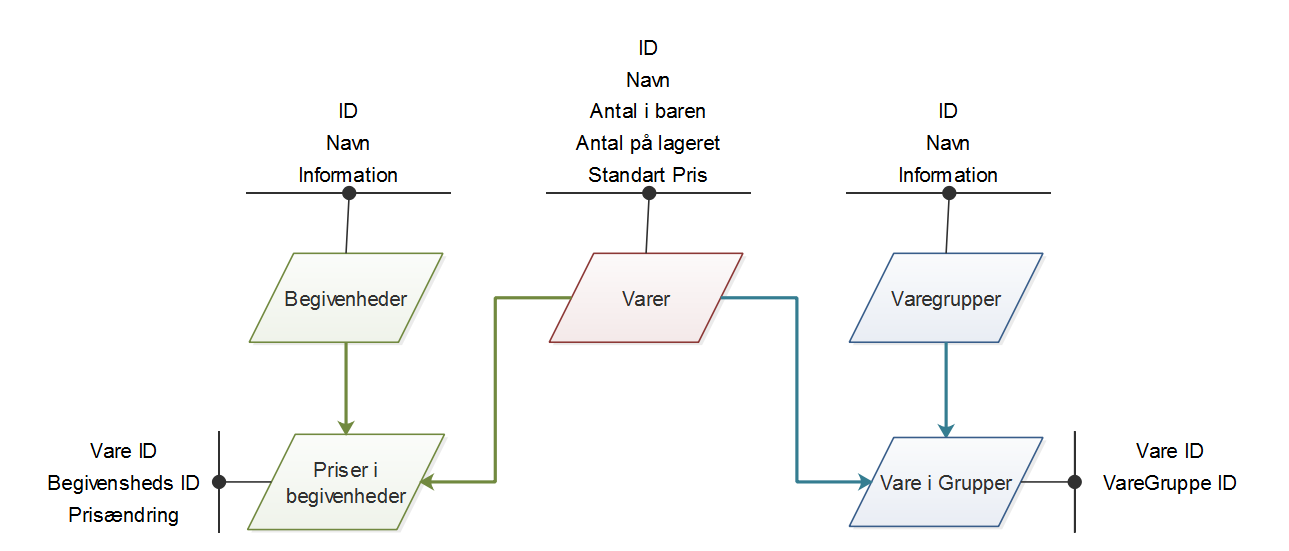
\includegraphics[width = \textwidth]{Database.png}
	\caption[Database]{Kommunikationen mellem tabellerne der i programmets backend.}
	\label{fig:database}
\end{figure}
 \noindent I hver class er der en række funktioner, som bruges til at søge og ændre i databasen. Flere af disse er predefineret i Django, men er ændret for at tilpasse projektets behov. \\
\begin{wrapfigure}{r}{0.5\textwidth}
	\vspace{-25pt}
	\begin{center}
		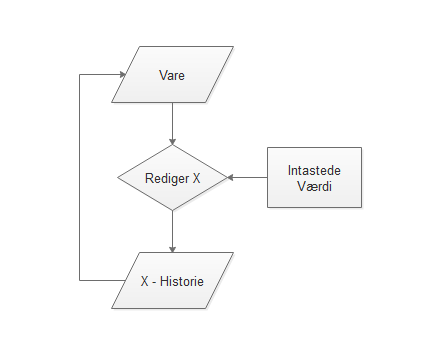
\includegraphics [width=0.48\textwidth] {ChangeValue.png}
	\end{center}
	\vspace{-25pt}
	\caption[Funktionsstruktur for at gemme ændring i tabel]{Den nye funktionsstruktur til at gemme en tabel-ændring. Denne funktion er skrevet for hver tabelværdi (substituer $X$ med felterne i de forskellige tabeller, som ses i figur \ref{fig:database}).}
	\label{fig:Change}
\end{wrapfigure}
\noindent Eksempelvis har Django en simpel måde, hvorpå man kan gemme nye værdier i databasen. Denne metode overskriver dog værdien, så historikken ikke findes. Dette var netop et af kravene fra kunden, som er løst ved at lave en tabel i databasen for hvert felt i de angivne classes i figur \ref{fig:database}. \\
Den benyttede funktion til at redigere et felt i en tabel i databasen ser ud som i figur \ref{fig:Change}, hvor en ændring gemmes i en særskilt tabel med tidsstempel og den nye værdi. \\
Det blev overvejet at lave en ny tabel hver gang, der blev foretaget en ændring. Tabellen skulle indeholde dato, tidspunkt og vareoplysninger. Dette fandt vi dog ville blive uoverskueligt at bruge for kunden, da det ved denne løsning krævedes, at man kendte ændringstidspunktet.

\subsection{Overvejelser omkring koden}
I dette projekt er der ikke gjort brug af nedarvning og interfaces som er beskrevet i \textbf{Agile} og \textbf{Code Complete} \cite{martin2006agile,mcconnell2004code}. Grundet kodens størrelse vurderede vi, at ikke megen tid ville blive sparet ved at benytte disse principper, selvom det ville have en gavnlig effekt ift. korrekte vaner, når der arbejdes på projekter.
% Det ville have været muligt at lave en modelklasse med eksempelvis historik -elementer som alle andre historikker arver fra. På samme måde er eksempelvis alle deletethis for Wares, Waregroups og Events af meget ens natur. Kodens størrelse har dog ikke givet indtrykket af at dette ville have sparet meget tid ift dette projekt, men mere haft en gavnlig effekt på korrekte vaner til fremtidige projekter. \\
% \indent Der er heller ikke oprettet interfaces for Models som kan tilgås af eksempelvis Views og Forms, hvor koden på samme måde ikke virker som af en størrelse hvor dette er stærkt nødvendigt.\\

\subsubsection{Kodekonventioner}
\noindent For at have et projekt, der er let at vedligeholde, er det nyttigt at aftale kodekonventioner internt i gruppen. Dette er for at sikre ensartethed i programmeringen. På denne måde bliver det altså lettere at læse koden. En kodekonvention er især nødvendig, når der er flere programmører på samme projekt, men en kodekonvention medvirker også til, at programmet bliver dokumenteret, så fremtidige programmører kan sætte sig ind i funktionaliteten. Derudover bliver koden mere overskuelig med et konsistent layout. En kodekonvention fjerner en del af den kompleksitet der er, når man skal sætte sig ind i programkode, som beskrevet i \textbf{Code Complete} \cite{mcconnell2004code}. \\
Variabelnavne, funktionsnavne og klasser er ikke blevet udviklet på baggrund af en fastlagt konvention, men det er forsøgt at benytte indsigten fra \textbf{Code Complete} \cite{mcconnell2004code} omkring navngivning af variabler og \textit{functional cohesion} for funktionskaldende.

\subsubsection{Refaktorering}
\noindent For at have et godt design er det vigtigt, at redesigne koden løbende for at kunne imødekomme nye krav og ændringer i funktionaliteten af programmet. Hver gang en ny funktion tilføjes, er det vigtigt at se på, hvordan designet kan ændres, så lignende fremtidige ændringer er lettere at implementere. Ved at gøre det sådan, kan man koncentrere sig om at finde en simpel løsning til det enkelte problem og redesigne løbende.

\subsubsection{Forhold mellem backend og frontend}
\noindent For at have et godt modulariseret design, bør valg af frontend være uden betydning for backend. Det bør også være muligt at anvende dele af backend til andre formål, men denne form for generalisering kan fjerne fokus fra slutproduktet, som her er et funktionelt program.
%Hvis et design skal være ordentligt modulariseret bør backend være ligeglad med hvilken frontend der anvendes. I mindre grad bør man også kunne tage en del af backend som eksempelvis wares og anvende til andre formål. Wares indeholder dog eksempelvis en funktion som "getopeningwares" der forholder sig til behovet for at registrere indeholdet for åbne varer, hvilket ikke nødvendigvis ville være relevant i et andet optællingssystem. Der er dog to indvendinger mod at skulle tage modulariseringen til den slags højder. For det første er det begrænset hvor meget ny kode der er i Wares relativt til blot at skabe et nyt djangoprojekt. For det andet kan man risikere at en sådan generalisering hurtigt kunne ende med at fjerne fokus fra slutproduktet (et funktionelt program) til fordel for designfilosofi.\\
Vi har forsøgt at holde backend og frontend adskilt. \texttt{Models.py} gør udelukkende brug af \texttt{exceptions.py} og Djangos underliggende biblioteker. \\
%\indent På trods af denne antagelse om hvad backend skal anvendes til er der dog ikke ellers en sammenblanding af backend og frontend. Models.py gør udelukkende brug af exceptions.py og Djangos underliggende biblioteker. 
Frontend kender til backendfunktionaliteterne og disse er ikke indpakket i et interface. Det er frontend, der tjekker, om baren er åben, selvom dette med fordel kunne være flyttet til backend. Ved at tjekke det i frontend kan det ske, at een bruger kan redigere oplysninger for en anden bruger, selvom systemet ikke burde tillade det. \\
Modulariseringen ville være gjort mere kompliceret ved at tjekke dette i backend, men det havde sikret et mere hensynsmæssigt program for kunden ud for de beskrevne krav. \\
Dette problem kunne modvirkes ved at pakke kommunikation mellem backend og frontend ind i et interface.
% Derudover udføres checks omkring hvorvidt baren er åben i frontend. Disse checks kunne med fordel flyttes til backend, da man ellers er i den problemstilling at et faneblad kan åbnes af een bruger mens en anden eksempelvis åbner baren. Muligheden for at redigere i oplysningerne for den første bruger vil dermed være tilstede selvom systemet ikke burde tillade det. Havde man flyttet disse checks til backend havde man yderligere besværliggjort modulariseringen men samtidigt sikret et mere hensigtsmæssigt program til den aktuelle kunde. Disse problemer kunne selvfølgeligt igen modvirkes ved at pakke kommunikationen mellem backend og frontend ind i et interface.

\subsection{Priser}
I forbindelse med projektet har vi haft adskillige overvejelser omkring prisopsætning, da der har været ønske om mulighed for at ændre dette baseret på den enkelte begivenhed.

\subsubsection{Uafhængige priser}
\noindent Under hver begivenhed kunne man have en særlig pris for varer og varegrupper, der var uafhængig af andre priser. Dette ville dog medføre, at alle priser skulle indtastes ved oprettelse af en begivenhed, og at en vare eller varegruppe kunne stå til 0 kr., hvis en indtastning manglede. \\
Vi fandt det mere hensigtsmæssigt, at systemet for varen eller varegruppen ville falde tilbage på en standardpris, hvis der ikke blev angivet en pris for den nyoprettede begivenhed. 
% Problemet blev så hvordan denne pris bedst kunne gemmes.

\subsubsection{Standardbegivenhed}
\noindent Til disse standardpriser kunne een af begivenhederne have rollen som standardbegivenhed, hvorfra standardpriserne kunne hentes til andre begivenheder. \\
Fordelen ved dette design er enkeltheden i konstruktionen, da det er en intuitiv tilgang til problemet "I denne begivenhed koster denne vare dette", men der er ligeledes uhensigtsmæssigheder.\\
For programmørerne ville der være den problemstilling, at det skulle afgøres, hvilken begivenhed, der var standardbegivenheden. Den førstoprettede begivenhed kunne vælges som udgangspunkt, men der kunne opstå fejl, hvis denne begivenhed eksempelvis blev slettet. \\
For kunden ville problemet opstå, når systemet havde flere begivenheder, og det var ønsket at ændre i prisen for en vare. Denne ændring skulle så foretages i alle begivenheder. Hvis der ikke altid var relation mellem standardprisen og begivenhedsprisen, kunne man dermed ende med et større vedligeholdelsesarbejde.

\subsubsection{Varespecifiseret standardpris} \label{VarePris}
\noindent Vi endte med at sætte en standardpris for en vare og lade begivenhedspriserne blive bestemt i forhold til denne pris. Der kan altså tastes $\pm \, x$ kr. i forhold til standardprisen ud for en vare i en begivenhed, hvor standardprisen benyttes ved manglende indtastning. \\
Hvis standardprisen reguleres, vil de begivenhedsbestemte priser reguleres tilsvarende. 

\subsubsection{Brugerflade}
\noindent  Til brugergrænseflasen er der fremstillet to forskellige variationer af prisfastsættelsen for begivenheder. \\
Den ene udregner den totale pris for en given vare i en begivenhed og viser denne, når 'liste over priser' vælges. Dette betyder, at man vil blive bedt om at sætte vareprisen for en begivenhed og ikke prisændringen, hvis prisen ønskes ændret. \\
Den anden benytter metoden som beskrevet i afsnit \ref{VarePris}, men her er det priser for varegrupperne, og altså flere varer der reguleres på een gang. \\
Her er vist noget af en klasse fra \texttt{forms.py}, hvor vi ser på standardprisen for en vare.
\begin{lstlisting}
class WareForm(forms.Form):
    wareid = 0
    name = forms.CharField(label='Varenavn', max_length=100, required=False)
    inbar = forms.IntegerField(label='Antal i bar', required=False)
    instock = forms.IntegerField(label='Antal paa lager', required=False)
    price = forms.IntegerField(label='Standardpris (kr.)', required=False)
    waregroup = forms.ModelChoiceField(queryset=Waregroups.objects.all(), required=False, 
                                       empty_label="Intet valgt", label="Varegruppe")

    def clean_price(self):
        price = self.cleaned_data['price']
        if (price == None):
            pass
        else:
            Wares.setstandardprice(self.wareid, price)

\end{lstlisting}

\begin{lstlisting}
def setstandardprice(wareid, newprice):
        ourware = Wares.getthis(wareid)
        ourware.standardprice = newprice
        ourware.save()
        Waresstdpricehistory.insert(wareid)
\end{lstlisting}

\subsubsection{Varegruppe- eller blot varespecifiseret priser}
\noindent Vi skulle her have konfereret med kunden om, hvorvidt det er et ønske, at lade varen bestemme prisen frem for varegruppen, som de har gjort indtil nu. Ønsker de at fortsætte med at lade varegrupperne angive priserne, kan dette dog implementeres uden de store omkostninger.

\subsection{Håndtering af sprut} \label{Sprut}
For at kunne opfylde kundens krav og ønsker, er det nødvendigt at systemet kan håndtere Caféen?s særlige optælling af sprut. Konkret skal vægten noteres for åbne sprutflasker.

\subsubsection{Underklasse}
\noindent Vi overvejede at lave en helt ny tabel i tabellen varer, så sprutflasker ville være en underklasse for varer. Denne mulighed blev ikke udforsket grundigt, da vi var usikre på simpliciteten af at operere med objekterne på denne måde.
%
%Man kunne lade sprutflasker som en underklasse for varer m.fl. potentielle underklasser senere. Altså lave en helt ny tabel i tabellen varer. Denne mulighed blev ikke udforsket grundigt, da vi ikke var sikre på hvor nemt det var at operere sådan med objekterne, når der reelt var tale om tabeller i en database. Vi var blandt andet usikre på, om der ville være utilsigtede konsekvenser for muligheden for at kunne hente alle varer baseret på id.

\subsubsection{Ekstra felter}
\noindent Vi overvejede at indsætte ekstra felter ved alle varer, hvilket kun ville være en enkelt ekstra værdi i tabellen. Da der er tale om et ekstra felt ved alle varer, vil der hurtigt kunne komme fejl, da det kun er i særtilfældet \textit{sprut}, at feltet skulle bruges. \\
For at løse dette kunne man lave en bool for sprut, som del af vareoprettelsen i kombination med ekstra felter. Der ville altså kun komme ekstra felter, når varen talte som sprut. Her ville der igen kunne opstå fejl ved ekstra felterne.
%\indent Dette virkede uhåndterbart for kunden da han så ville have et rastfelt ud fra alle varer og hvis priserne for de åbne varer skulle håndteres korrekt, kunne man nemt ende med mange ekstra oplysninger for en vare. \cite{mcconnell2004code} Hvis dette skulle håndteres kunne man nemt ende med et brud på \textit{Code Completes} design-filosofi om flags.\\
%\indent \textbf{Varegruppe med særlige egenskaber}\\
%Man kunne lade sprut-egenskaberne være bestemt af varegruppen. Man kunne dog dermed risikere at klasserne blev bundet for tæt sammen og de ekstra felter for vareoplysninger skulle stadig inkluderes i varen selvom de ikke var synlige for kunden. Hvordan varegruppen skulle noteres som en sprutvaregruppe og om dette var reversibelt kunne også give problemer længere henne i udviklingen.

\subsubsection{Oprettelse af (åben) vare}
\noindent Vi endte med at lave muligheden for at oprette en sjatvare, når en ny vare oprettes. Dette har betydet, at vi blot skulle tilføje en funktion, der kopierer de indtastede værdier for den oprettede vare, og tilføjer "(åben)"\, efter navnet. Funktionen beder om en ny enhedspris for denne vare. I frontenden ses en tjekboks under vareoprettelsen, som sender brugeren videre til oprettelsen af (åben)varen ved afkrydsning af denne boks. \\
Ved optælling vil disse varer blive listet ved siden af hinanden. Optællingsenheden er op til kunden, som blot skal indtaste den nye enhedspris. Det kan eksempelvis opgøres i gram, hvor prisen per gram så skal noteres ved oprettelse. \\
Denne løsning krævede, at vi foretog en ændring i vores åbne/lukke funktion, hvor vi hidtil kun har vist varer, der var på lager, hvor (åben)varer ikke ville figurere på lukkelisten, hvis denne vare ikke var åben ved åbning af baren. Dette er løst ved at medtage varer, der i navnet indeholder strengen "(åben)". \\
%
%\indent Der er i øjeblikket ingen checks for, om den åbne vare allerede eksisterer ved navn og derfor ikke vil blive oprettet af systemet. Ligeledes bliver brugeren ikke gjort opmærksom på varens natur som sprutflaske, kagepakke eller hvad kunden ellers kunne ønske at opgøre i lukket og åbne varer i fremtiden. \\
Generelt for overvejelserne af denne problemstilling skal det nævnes, at vi følte os usikre på, hvordan denne implementering var ønsket. De efterfølgende mailkorrespondancer gjorde os ikke klogere på kundens ønsker, da vi havde indtrykket af, at vi talte forbi hinanden. Grundet deadline besluttede vi os for ovenståede løsning på baggrund af egen intuition, selvom et fysisk møde med kunden havde været mere praktisk i en udviklingssituation. Dette stemmer også overens med det agile princip om at arbejde fysisk sammen med en kunderepræsentant, som beskrevet i \textbf{Agile} \cite{martin2006agile}.

\subsection{Håndtering af vareændringer bagudrettet}
Kunden har haft ønske om at kunne se tidligere oplysninger for varerne, også kaldet historik.
% Et af de ikke trivielle behov for kunden var ønsket om at have en mulighed for at se hvad et element i databasen havde haft af oplysninger tidligere. Normalt vil et databaseelement ikke opbevare oplysninger om tidligere stadier. Samtidigt ønskede vi ikke at disse tidligere oplysninger kunne påvirke systemet i normal produktionssammenhæng.

\subsubsection{Fil med ændring}
\noindent En måde at løse dette på, var at lade hvert element blive skrevet til en fil med alle oplysninger før og efter ændring sammen med tidspunktet herfor. Implementeringsmæssigt var dette en god løsning, men for fremtidig udvikling kunne der opstå problemer, da der er ønske om at systemet skal kunne integreres med et regnskabssystem. Denne tekstbaserede udskrift ville umiddelbart være besværlig at benytte i et sådant regnskab.
% En tekstbaseret udskrift ville være meget svær at udnytte til et sådant regnskab og ville kræve mange regulære udtryk som hurtigt kunne kræve meget lange køretider for at give et svar.

\subsubsection{Tabeller med ændringer}
\noindent Vi overvejede at foretage disse udskrifter til en databasetabel, hvor varens felter eksempelvis kunne blive gemt ved hver foretaget ændring. Dette ville inkludere mange uændrede data, grundet kopiering, da en vares navn sandsynligvis ikke ville blive ændret samtidig med en optælling. 
% Der var også en bekymring for hvordan disse ekstra oplysninger kunne påvirke et fremtidigt regnskabssystem.

\subsubsection{Felt historik}
\noindent Vi valgte at oprette en historikklasse for hvert felt i tabelobjekterne. Dette skabte mange ekstraklasser i \texttt{models.py}. \\
Disse historikker skal kunne sammenlignes baseret på publiceringsdato, og dermed kan prisen for en vare for en begivenhed eksempelvis findes og ganges med antal solgte varer for at finde indtægten for en given dag. \\
% Dette skabte mange ekstraklasser i models.py, men da deres funktionalitet indtil videre er begrænset, var de nemme at sikre til en nogenlunde tryghed over koden. Det er så meningen at disse historikker kan sammenlignes baseret på deres publiceringsdato og man dermed kan finde eksempelvis prisen for en vare for en begivenhed og gange med antallet af solgte varer for at finde indtægten en given dag.
Dette er et eksempel på en klasse i \texttt{models.py}, hvor der ses på historikken for varerne i baren.
\begin{lstlisting}[language=Python]
class Waresinbarhistory(models.Model):
    id = models.AutoField(primary_key=True)
    pub_date = models.DateTimeField(auto_now=True)
    wareid = models.IntegerField(default=0)
    inbar = models.IntegerField(default=0)
    
    def __str__(self):
        information = "Vare med ID #" + str(self.wareid) + ", navn" + self.warename + 
                       " har " + str(self.inbar) + " varer i baren"
        return information
    
    def insert(warid):
        ware = Wares.getthis(warid)
        warehis = Waresinbarhistory()
        
        warehis.wareid = warid
        warehis.inbar = ware.inbar
        warehis.save()        

\end{lstlisting}

\pagebreak[3]

\section{Afprøvning} \label{Afprovning}
Det er vigtigt for et softwareudviklingsforløb at teste/afprøve ens software. Afprøvning er centralt for at opfange fejl og mangler i koden, og for at sikre, at programmet virker efter hensigten. Derudover undersøges det, om koden lever op til de stillede krav. Grundig gennemtestning hjælper til at eftervise programmets robusthed og pålidelighed. Det estimeres i \textbf{Code Complete} \cite{mcconnell2004code}, at et typisk softwareudviklingsprojekt vil bruge 8-25\% af tiden på testing.  \\ \\
I dette afsnit vil vi gennemgå de overvejelser, vi har haft i forbindelse med forskellige tests af systemet. Afsnittet vil omhandle både backend og frontend tests. Vi vil reflektere over brugen af både de manuelle og automatiske test samt overvejelser og brug af testfunktioner. \\
Ordene 'teste' og 'afprøve' vil i dette afsnit blive brugt som synonymer. 

\subsection{Overordnede overvejelser for afprøvning}
For at kode agilt er det ideelt at lave tests inden den egentlig kode er skrevet. Disse tests medvirker, at man har dokumentation for koden allerede inden, den er skrevet, som ikke bliver forældet. Man tvinges til at gøre grundige overvejelser over, hvad man ønsker at skal kunne, og disse tests laves således til at mindske antallet af fejl, der kan opstå i koden. \\
Denne form for testing, \textit{test-first}, er der dog udfordringer ved, som vi har oplevet i forbindelse med udviklingen af vores kode. For at komme godt igang med kodeprocessen skulle teknologien læres at kende, og i den forbindelse blev dokumentationsdokumenterne brugt som udgangspunkt. Dette medførte brugbar kode, som der ikke var udviklet \textit{test-first} for. Det bryder altså med \textit{test-first} mentaliteten, men medvirkede til en effektiv start i et hidtil ukendt udviklingsmilø. \\
\indent Vi fandt, at ved brugen af \textit{test-first} kommer der et brud på udviklerens flow ved at skifte mellem tests og funktionel kode. I udforskningszonen kan det føles som et dobbeltarbejde, at skulle skrive testkode, hvorfor koden er skrevet, som vi tænkte bedst for så at skrive testfunktioner til at teste alle tænkt mulige scenarier. \\
\indent Vi har oplevet variation i, hvor godt koden kunne testes. De automatiserede tests er blevet udviklet i forbindelse med backenden, men Django-dokumentationen \cite{DjangoDoc} gav ikke umiddelbart beskrivelser af, hvordan man lavede tests for view-metoder. Beskrivelserne fra dokumentationen fokuserede på Djangos Form- og View-klasser, men disse er blevet benyttet i begrænset omfang i projektet.


\subsection{Unit tests}
Unit testing er afprøvningen af klasser, metoder og andre afgrænsede programmer, der er skrevet af en eller flere udviklere, hvor afprøvningen foregår enkeltvist og isoleret fra det samlede system (\textbf{Code Complete} \cite{mcconnell2004code}). \\
Vi har løbende i processen lavet tests for funktioner/klasser, når disse er blevet implementeret. Dog er implementeringerne i 5. iteration prioriteret højere end tests af implementeringerne. Ifølge \textbf{Code Complete} \cite{mcconnell2004code} er der en tendens til, at programmører er for optimistiske omkring egenvurdering af dækket kode, hvorfor vi vil skønne, at omtrent 50\% af vores kode er testet, da man jo altid kan teste lidt mere. \\
\indent De anvendte testcases er designet sådan, at hver funktion principielt kun afdækker een funktionalitet i programmet, og med denne bagtanke er testene for hver funktion rimeligt udvidede. Frem for bare at teste een ting per test, kan adskillige scenarier testes i en testfunktion, men hvor fokus i alle scenarierne er at afprøve den relevante funktion. Dermed kan der være adskillige asserts per test. Vores unit tests er automatiserede, som beskrives i afsnit \ref{AutomatiseredeTests}.

\subsection{Acceptance tests}
Acceptance tests er modsat unit tests en måde at teste det samlede system på frem for de enkelte programdele. \\
Acceptance tests er afprøvninger af systemet, som brugeren ville se systemet. Dette betyder altså for os, at afprøvningen er af det webbaserede lagersystem, hvor der så udføres black-box tests. Dvs. at der ikke er kendskab til den interne implementering af funktionaliteten. Kunden har i begyndelsen specificeret, hvornår en use case er implementeret korrekt, hvilket kan betyde at der er flere acceptance tests per use case \cite{martin2006agile,mcconnell2004code}. \\
Kravene til lagersystemet er beskrevet i afsnit \ref{Krav}, hvilket vores acceptance tests er bygget ud fra. En stor del af disse tests er udført som manulle tests som beskrevet i afsnit \ref{ManuelleTests} og \ref{BrugerfladeTests}.


\subsection{Automatiserede tests} \label{AutomatiseredeTests}
Automatiserede tests giver fordele for vedligeholdelse og arbejdsproces omkring projektet, som beskrevet i \textbf{Code Complete} \cite{mcconnell2004code}
\begin{itemize}
	\item Det fjerner på sigt en stor arbejdsbyrde fra den enkelte programmør, der slipper for at teste programmet manuelt.
	\item Det giver en voksende base af tests, som kan bruges af fremtidige programmører, og når først en test er automatiseret, kan den bruges af alle uden en større indsats eller viden om testen.
	\item Automatiserede tests er fejlmæssigt overlegne sammenlignet med manuelle tests. Mennesker har en tendens til at lave fejl, f.eks. ved at taste input forkert. Det gør den automatiserede test ikke. Mennesker bliver trætte og ukoncentrerede efter at have gennemset et stort antal tests. Det gør en computer ikke. En programmør kan ikke let i praksis køre tusinder af tests manuelt - det kan en computer.
	\item Automatiserede tests kan blive kørt ofte og hurtigt, modsat manuelle tests.
	\item Man findere hurtigere fejl ved at bruge automatiserede tests, når man udvikler på programmet. Dette skyldes, at deres hurtige anvendelighed gør, at man hver gang en ny funktionalitet er implementeret kan teste dens gyldighed i forhold til de etablerede tests.
\end{itemize}
Automatisering af tests er altså en fordel, når projektet i fremtiden skal arbejdes videre på, da disse tests hurtigt vil kunne fortælle, når en ændring giver fejl i det eksisterende system. Ligeledes er det en fordel for robusthed, da automatisering kan bruges til at skalere tests op. \\
\indent De automatiserede tests er sat ind i filen \texttt{cafeen/tests.py}. Disse tests er blevet kørt ved at benytte kommandoen '\texttt{python tests.py test}'. Den anvendte \texttt{tests.py} har fået indsat koden fra \texttt{manage.py}. Dette er reelt ikke nødvendigt, men har fået lov til at overleve, fordi andre dele af koden har haft større prioritet. \\
% Django har allerede leveret en tests.py fil i cafeen/polls/tests.py, men denne blev ikke benyttet til at starte med og siden har den nuværende test-fil fået lov at overleve fordi der altid har været større prioriteter i arbejdet. 
\indent De automatiserede tests dækker kun et subset af koden. Da View-funktionerne og Form-klasserne blev dannet, var det ikke afklaret, hvordan disse skulle testes, da en del af testen kræver en form for simuleret bruger-input. \\
Vanen med at danne tests blev brudt i takt med at afleveringsfrist nærmede sig. Dette har medført, at der ikke er oprettet automatiserede tests til klasser som \texttt{Openandclose} i \texttt{models.py}. \\
\indent De automatiserede tests er blevet udført samme dag, som den respektive kode, der skulle testes. De automatiserede tests opdagede fejl, som var opstået af andre rettelser. 
% Derudover mindskede det problemerne ved det kodegenbrug, som fandt sted ved designet af backend. Ved kopieringen af visse funktioner hændede det at den forkerte historik blev kaldt. En sådan fejl kunne nemt have sneget sig igennem systemet hvis ikke de automatiserede tests fangede problemet med det samme.

\subsection{Manuelle tests} \label{ManuelleTests}
I visse situationer blev der ikke lavet automatiserede tests til vores software. Disse tests har da været manuelle, som eksempelvis har bestået af \texttt{print()}-kald indlagt i koden, for at se om kodens \textit{conditionals} blev eksekveret korrekt. \\
Disse tests grænsede til debugging, men er også benyttet til at klarlægge Djangos funktionaliteter under læringsprocessen. \\
\indent Vi har også testet softwaren manuelt ved at indtaste forskellige værdier i frontendsystemet. Dette blev gjort for at undersøge, om konsekvenserne ved indtastningerne svarede til det forventede. \\
Disse manuelle tests minder om brugerfladetests, men fokus var ikke nødvendigvis i brugerfladen, men derimod funktionaliteten. \\
Fælles for disse metoder er, at de ikke permanent tester koden, og at de nemt ender med at tage mere tid, end man kunne forvente fra automatiserede tests. Metoderne har dog den fordel, at de tvinger programmøren til at reflektere over, hvad koden skal kunne og kan hjælpe med at lære, hvordan de underliggende biblioteker fungerer.
% Her tænkes bla. på request.POST beskrevet under debugging.

\subsection{Brugerfladetests} \label{BrugerfladeTests}
Det var nødvendigt at indtaste værdier gennem den udviklede brugerflade, som del af de manuelle tests. Dette har givet en indsigt i funktionalitet af backend og frontend og givet mulighed for reflektion over slutbrugerens oplevelser og muligheder, såsom hvor mange klik der skal bruges for ønsket effekt. \\
Brugerfladetesten fangede en problemstilling i det overordnede design, der ikke var blevet overvejet tidligere eller fanget af de automatiserede tests. I forsøget på at skifte en vares associerede varegruppe, blev denne blot tilføjet en liste af associerede varegrupper. Når varens varegruppe skulle findes, fik man dog kun det første resultat, hvilket betød at det ikke var muligt for brugeren at ændre varegruppeassociationen efter første valg. Dette tvang os til at afgøre, om det gav mening at en vare kan tilhøre flere varegrupper. Vi har ikke haft brugerfladetests af egentlige brugere. Dette kunne have hjulpet udviklingen af brugerfladen, men vores fokus har været en funktionel backend.  

\subsection{Debugging}
I løbet af projektet har vi benyttet os af debugging til at rette fejl i koden. Her følger et eksempel på dette. \\ \\
Ved brugerinput blev de indtastede værdier i nogle situationer ikke modtaget. Tidligere havde der været problemer med Django-undtagelserne \texttt{AttributeError} og \texttt{KeyError}. Disse kom eksempelvis når kun nogle informationer var indtastet. Da disse fejl kom i starten af implementereingen af brugergrænsefladen, var \texttt{views}-metoderne ikke tilpas forstået endnu. For ikke at gå i stå blev disse fejl ikke rettet/fundet i første omgang. I stedet blev arbejdet med \texttt{views}-metoder droppet for at bevæge sig over i \texttt{views}-klasser og \texttt{form}-klasser i stedet. Da dette heller ikke gav den ønskede brugerflade, blev metoderne genanvendt med lappeløsninger på problemet, dog med et \texttt{\#TODO:} skrevet ind i koden for at markere at denne kode ikke var korrekt udformet. Relativt sent i projektet blev det opdaget ved et tilfælde at \texttt{request.POST} krævede en yderligere conditional end tidligere planlagt. Den manglende overvejelse skyldtes en misforståelse af, hvornår Django eksekverer sin kode. \\ \\
Implementeringen af at kunne bestemme varegruppers priser baseret på en begivenhed var blandt de sidste funktionaliteter, der blev tilføjet til brugerfladen. Enkelte varer kunne allerede prisjusteres, så opgaven blev vurderet som relativt triviel. Da implementeringen blev testet endte Django dog i flere tilfælde med at give en \texttt{IndexError}. Det var ikke muligt at finde fejlen blot ved at følge loggen og da problemet inkluderede førstnævnte problem, opstod der et behov for at dykke ned i, hvad der skete i koden.\\
\indent Første skridt var at udkommentere en række af de kald, som \texttt{view}-metoden gjorde brug af, således at fejlens mulige placeringer kunne isoleres delvist. \\
\indent I andet skridt blev \texttt{print}-statements indsat i \texttt{view}-metoden ved hvert \texttt{if} og \texttt{else} for at kunne afgøre, om koden opførte sig som forventet. Misforståelsen fra førstnævnte blev fundet ved denne metode, men ellers fungerede koden som forventet. \\
\indent I tredje skridt blev \texttt{view}-metodens kald genindført og den kaldte \texttt{form}-klasse blev i stedet udsat for udkommenteringer og \texttt{print()}-funktioner. I stedet for at printe, at koden kom til et bestemt stadie i koden, var der dog her større interesse for hvilke \texttt{id}-værdier, som blev kaldt, da dette øjensynligt var årsagen til den fundne \texttt{IndexError}. Den anvendte hypotese på dette tidspunkt var, at \texttt{WaresInWaregroup}-relationen ikke korrekt havde slettet en relation, da en vare blev slettet. Dette kunne blandt andet være sket i testdatabasen, fordi denne ikke var blevet renset under udviklingen af funktionaliteten.  \\
\indent Blandt de givne resultater kom et vareid op der var blevet slettet tidligere på dagen. Dette virkede umiddelbart til at bekræfte hypotesen, men varen var ikke registreret i \texttt{WaresInWaregroup}. En kortlægning af relationerne i \texttt{WaresInWaregroup} viste, at der her ikke var nogen fejlregistreringer. Samtidig var det muligt at se, at der ikke var sammenhæng mellem de resultater man fik ved at tilgå \texttt{WaresInWaregroup} direkte, og så den måde det foregik på og de resultater der kom fra \texttt{form}-klassen.\\
\indent Under endnu en granskning af \texttt{form}-klassen viste det sig, at et af variabelnavnene var forkert. En variabel var sat til \texttt{ware}, selvom det var en samling af \texttt{WaresInWaregroup}-objekter. Dette havde skabt en misforståelse senere i koden, hvilket bevirkede at \texttt{ware.id} ikke havde fundet varens id, men derimod den id, som \texttt{WaresInWaregroup}-objektet havde. Ved at ændre \texttt{ware} til \texttt{warerelation} og \texttt{ware.id} til \texttt{warerelation.ware.id} forsvandt alle uoverensstemmelserne. 

\pagebreak[3]


\section{Proces} \label{Proces} % i udviklingen}
I dette afsnit vil vi komme ind på gruppens proces i forløbet. \\
For at producere brugbar software har fokus været på agil udvikling, hvor der er flere effektive processer. Vi vil forsøge at klarlægge, hvorvidt udviklingsprocessen har overholdt idéerne for agil udvikling. Dette gøres med udgangspunkt i det agile manifest \cite{martin2006agile}.
\begin{enumerate}
    \item \textbf{Release early, release often} \\
Dette punkt kan være svært at besvare med sikkerhed, da tidshorisonterne for softwareprojekter kan variere meget. Fire måneders udvkling mellem hvert release kunne kvalificeres som hyppigt sammenlignet med rejsekortet, men gruppens evne til at overholde kravet relativt til to-ugers del-iterationer har været mindre frugtbart. Dette har været påvirket af den manglende brugerflade, som har gjort det uklart i gruppen, om en funktionalitet har været fuldt implementeret. Set fra brugerens synsvinkel er backend sjældent et færdigt produkt.

    \item \textbf{Welcome change, even late in development} \\
Forandringerne har ikke været så markante, da kunden allerede fra starten havde et godt kendskab til egne behov og ikke kom med pludselige skift fra den oprindelige specifikation i løbet af processen. Et eksempel på pludselige skift kunne dog være, at muligheden for at indsætte kommentarer ved åbning og lukning var blevet glemt i designet, selvom det var skrevet ind som et use case. Da denne fejl blev opdaget tog det mindre end en dag at implementere i frontend, backend og historik. Vi kan dermed sige at vores system kan håndtere ændringer og tilføjelser, også senere i processen.
% Vores svar fra kunden for håndtering af sprutflasker førte ikke til en 
%ændring af vores oprindelige tanker for implementationen. Dog blev de oprindelige designovervejelser vendt som optakt til mailkorrespondancen. \\

    \item \textbf{Deliver working software frequently} \\
Et princip for GitHub uploads var, at koden skulle fungere, inden man uploadede til master branchen. Derudover blev der løbende tilføjet funktionaliteter. Det var dog først i slutningen af projektet, at funktionaliteten kunne ses som brugbar i en produktionssammenhæng. 
 
    \item \textbf{Businesspeople and developers must work together daily} \\
Dette er ikke blevet overholdt, men ville heller ikke have været et realistisk krav for en konstrueret opgave. 

    \item \textbf{Build projects around motivated individuals. Trust that they get the job done} \\
Dette kan være svært at tilpasse med en konstrueret opgave udenfor en forretningssammenhæng, som i punkt 4.
 
    \item \textbf{The most efficient communication is face to face} \\
Dette har vi i gruppen ikke været gode nok til at udnytte og dette har formentligt været en alvorlig hæmsko i udviklingen. Mailkorrespondancerne i projektet har krævet en latenstid, man aldrig ville opleve med direkte kontakt. 
En væsentlig årsag til disse problemer været bundet i forsøget på at udvikle projektet imens andre fag også krævede tid. Dette ville i en professionel sammenhæng svare til at medlemmerne havde for mange forskelligartede opgaver udenfor deres rolle i projektet.

    \item \textbf{Working software is the primary measure of progress} \\
Dette ligger i fin tråd med beslutningen om at nedprioritere andre dele af kurset til fordel for at få lagertællingssystemet til at virke. Dog har vi formentligt haft et lidt for stort fokus på dette punkt i forhold til punkt 6, da hyppige møder kunne have øget motivationen til at arbejde på koden.

    \item \textbf{Should promote sustainable development} \\
Med undtagelse af gruppens inaktive periode og forsøget på at få alt på sporet igen, har der været et nogenlunde jævnt tempo.

    \item \textbf{Have attention to good design continuosly} \\
Der har ikke været fokus på at undgå kodegenbrug i projektet. Første prioritet har været at få kode til at virke, og derefter om man kunne gøre det mere hensigtsmæssigt. Hvis ikke koden blev udviklet hensigtsmæssigt i forhold til kodegenbrug, er det blevet noteret til senere rettelser. Dette er tilfældet for især \texttt{views} og \texttt{templates}, selvom klasserne i \texttt{forms.py} også kan forventes at skulle refaktoreres.

    \item \textbf{Maximise the amount of work not done} \\
Som det bliver beskrevet i \textbf{Agile} \cite{martin2006agile} stiller vi os mildt tvivlende for, om dette nødvendigvis er en god idé i alle sammenhænge. \textbf{Code Complete} \cite{mcconnell2004code} stiller sig også kritisk for denne filosofi. I projektet var der flere krav end blot at have et optællingssystem. Da disse krav også skulle kunne indfries på et tidspunkt, gav det mening at diskutere startdesignet med det udgangspunkt, at man skulle kunne bygge videre mod den fremtidige funktionalitet. Designet handlede derfor i høj grad om at
    \begin{enumerate}
        \item Sikre at man ikke spændte ben for sig selv på lang bane
        \item Opdele opgaver i uafhængige underopgaver, så det var muligt for flere at arbejde uden at frygte det var til gene for andre
        \item Fastlægge rækkefølgen af implementeret funktionalitet ift. afhængigheder og brugbarhed.
    \end{enumerate}
    
    \item \textbf{The team should be self-organizing} \\
Dette har i høj grad været tilfældet for vores gruppe, men ikke alle konsekvenserne har nødvendigvis været positive. Eksempelvis havde gruppen ikke valgt en projektleder, hvilket i \textbf{Geek} \cite{fitzpatrick2012team} beskrives som en sikker vej til inaktivitet, hvilket gruppen oplevede i en periode. Gruppen er dog nået i mål, uden styring udefra. 

    \item \textbf{The team reflects and retunes regularly} \\
Som for punkt 1 er succes indenfor dette afhængigt af, hvilken målestok man sætter. Den oprindelige rollefordeling viste sig uhensigtsmæssig, men håndteringen af Mohammeds forsvinden (beskrives yderligere i afsnit \ref{Diskussion}) samt rollen for testskrivning, brugeradfærd mm. var reflektioner, som vi endte med ikke at have tid til at indstille os efter. Havde der været yderligere arbejde for at få regnskabssystemet til at virke, ville dette naturligvis have årsag til at arbejde med ændret rollefordeling.
\end{enumerate}

\subsubsection*{Konklusion}
\noindent Med tidsfristen taget i betragtning, har gruppen som helhed formået at overholde flere af de fastsatte principper for agil udvikling, som bliver fremhævet i manifestet. Blandt de punkter, som gruppen ikke har været gode til at overholde, er nogle baseret på manifestets fokus på egentlig virksomhedsproduktion og ikke et førsteårsprojekt.

\subsection{Kundekontakt}
Det havde været ønskeligt at have fysisk kontakt med Jenny, både i forhold til afklaring af funktioner og i form af egentlige brugertests. Kommunikationen foregik via mail, se bilag \ref{Mails}. I afsnit \ref{Diskussion} %og ved relevante problemstillinger,
vil gruppens håndtering og tolkning af disse svar blive beskrevet. % samt sammenstillet med det endelige produkt. \\


\subsection{Gruppearbejde}
Her vil gruppearbejdet blive beskrevet for hele processen.

\subsubsection{Delaflevering 1}
\noindent I perioden op til delafleveringen fik gruppen lavet en designskitse, udviklet use cases, og fik en idé om, hvor meget der kunne nås på den tid, projektet varede. Gruppen designede med henblik på, at opgaven kunne deles op i mindre delområder, så vi bedst muligt undgik dobbeltarbejde. \\ \\
Efter aflevering af delaflevering 1 var gruppen til møde med instruktorerne. Vi blev rost for vores fremgang, men fik råd og stillet krav til fremtidigt arbejde
\begin{itemize}
    \item Vi skulle arbejde med seperate GitHub-branches og merge disse for at få en korrekt forståelse af arbejdet med GitHub.
    \item Vi skulle fortsætte med grafer og diagrammer som visuel vejledning i vores delafleveringer.
    \item Vores user stories og use cases var velprioriterede og veludformede.
    \item Vi blev mindet om, at det er vigtigt at skrive programmeringstimer ind for hvert sprint, og at dette skulle inkludere, hvorvidt arbejdet havde været for \textit{must-have} eller \textit{nice to have} funktionaliteter.
    \item Vi blev bedt om at lave mødereferater for vores møder. Disse skulle have fokus på, hvad vi nåede og ikke nåede samt hvorfor dette var tilfældet.
    \item Vi blev opfordret til at skrive idéer og mails til Jenny ind i delafleveringerne, så det kunne noteres i vores fremgang. 
    \item Til sidst blev det krævet, at alle gruppemedlemmer skulle bruge PyCharm.
\end{itemize}

\subsubsection{Delaflevering 2}
\noindent Grundet lukkedage og sygdom blev gruppens muligheder for at arbejde på projektet mindsket kraftigt. Mødet efter påskeferien blev derfor primært brugt på at indhente arbejde på delaflevering 2 samt kort oprids af den begrænsede fremgang. Der blev ikke aftalt en konvention for placering af funktioner i forhold til Djangos struktur, så det var endnu ikke muligt at lave meningsfulde automatiserede tests, og delingen på GitHub var dermed også rodet. Mødet blev også påvirket af Nicolais første GitHub-problem, som formentligt var en konsekvens af ikke at bruge PyCharm, hvilket besværliggjorde merging.
%\begin{figure} [H]
%    \centering
%    \includegraphics [width=0.8\textwidth] {GitProblem.png}
%    \caption{Denne figur viser Nicolais problemer med Git, man kan se at Git har tilføjet en af PyCharm forståelig kode.}
%    \label{fig:GitProblem}
%\end{figure}

\subsubsection{Delaflevering 3}
\noindent Ligesom i påsken var ugerne lige før og under eksamensperioden for blok 3 præget af et begrænset fokus på softwareudvikling. Det var ikke muligt at samle gruppen til et fællesmøde, men blev i stedet delt op i enkelt og pararbejde. En konvention for kodeplacering endte med at blive besluttet ad-hoc.

\subsubsection{Delaflevering 4}
\noindent Den lange dødvandsperiode for gruppen havde opbrudt rytmen for gruppearbejdet. Forsøget på at etablere en rytme igen blev hæmmet af Mohammeds manglende svar på mailkorrespondancerne, da alle andre medlemmer af gruppen dermed ventede for længe på bekræftelser. Konsekvensen var, at Nicolai endte med at tage en spurt i udviklingen af koden uden gruppebeslutninger. De næste par møder var præget af også at få nået delafleveringen. Erfaringer med kodeopbygnng blev derfor kun gennemgået på et overordnet plan. \\
Det blev droppet at få Mohammed til at komme tilbage til gruppen, selvom vi fortsat var åbne for at han kunne komme tilbage.\\
Arbejdet på frontenden med den nu udviklede backend, skulle dermed genskabes på ny, da Mohammed ikke havde lagt sin fremgang med brugerfladen op på GitHub. \\ \\
Gruppemøder omhandlede dels at få etableret et fornuftigt design for varepriser, en diskussion af implementeringen af historik og hvordan vi kunne skabe en fornuftig frontend. \\
Gruppens arbejdsperiode omkring påske samt Mohammeds forsvinden gjorde det nødvendigt at omprioritere arbejdet. Arbejdet på fagets ikke-obligatoriske aktiviteter blev kraftigt neddroslet og forsøget på at få en brugerflade til at køre blev opprioriteret. Djangos struktur viste sig ikke at passe fuldt ud til vores behov, så denne proces krævede en del ny indlæring af den bagvedliggende struktur. Dette medførte noget ikke fuldt ud funktionel kode, der derfor ikke blev delt på GitHub med det samme. \\
Denne manglende synkronisering førte til det andet GitHub-problem for Nicolai, med et tab af 200-500 linier kode. Problemer med at merge med GitHub gjorde, at Nicolai lavede en backup inden han så kørte en \textit{clean}. Denne rengøring søgte dog hele computeren igennem, og slettede dermed også backuppen.
\pagebreak[3]

\section{Diskussion} \label{Diskussion} % af projektarbejde}
Dette afsnit kan opfattes som det opfølgende afsnit. Her vil vi gennemgå de sidste faktorer i projektet, samle op på tidligere gennemgåede punkter i arbejdet og beskrive, hvad vi er stødt på af udfordringer.

\subsection{Gruppen}
Vores gruppe blev dannet til første holdundervisning, hvor vi fandt sammen ved, at ingen af os kendte nogen. Ingen af os er førsteårsstuderende, og gruppen består af to dataloger og to fysikere.
\subsubsection{Team kontract}
\noindent Vores team kontract er en række normer, som vi ville overholde i gruppen. Kontrakten er brugt som en rettesnor, hvor vi inden projektets start lavede aftaler og overvejede arbejdsfordelingen. \\
Vi har i den forbindelse fulgt HRT-princippet (\textbf{Geek} \cite{fitzpatrick2012team}), hvor vi det har været vigtigt at udvise ydmyghed (Humility), respekt (Respect) og tillid (Trust) over for sin gruppe. \\
I den forbindelse talte vi i gruppen også om tidligere samarbejder, som alle havde en vis erfaring med. Dog var denne form for samarbejde ny, da der var tale om et større projekt og en større gruppe.
\subsubsection{Fordeling af opgaver i gruppen}
\noindent Da vi dannede gruppen, talte vi om forventninger til, hvor meget vi hver især forventede at kode, hvor vi også talte meget om de enkelte gruppemedlemmers kodeerfaring, hvilket også blev inkluderet i team kontrakten. \\
Alle gruppemedlemmerne forventede at kode noget, men det var tydeligt, at det var datalogerne, der havde den største interesse i at kode, og at fysikerne havde det fint med at kode lidt, men skrive mest på delafleveringerne og den endelige rapport. \\
Efter denne klarlægning blev følgende opdeling lavet:
\begin{itemize}
    \item Nicolai skulle have backend som primært ansvar.
    \item Mohammed skulle have frontend som primært ansvar.
    \item Søren skulle have overblik over begge områder og sikre at vi ikke afveg for meget fra designet. 
    \item Camilla skulle have kundekontakt og rapportskrivning som primært ansvar. 
\end{itemize}
Ansvarsopgaverne havde ikke til formål at begrænse bidrag hos en andens ansvarsområde, men blot sikre at hvert medlem i gruppen kunne få lov til at fokusere på og have ansvar for det givne område. \\ 
Disse ansvarsområder skulle have været aftalt igen på ny, som vi løb ind i udfordringer. Dette overblik manglede dog på tidspunkterne, hvor der i stedet blev arbejdet på kode og afleveringer. \\
\indent Opgavefordelingen (kode/skrivning) har altså ikke været til gene for nogen, men derimod var opgavefordelingen noget vi havde aftalt fra start, og der har generelt været en meget god stemning i gruppen.

\subsubsection{Manglende gruppemedlem}
\noindent Fra anden delaflevering, omkring påske, hørte vi pludselig ikke længere fra Mohammed, og selvom vi har prøvet at kontakte ham, har vi ikke fået svar. Derfor har vores arbejde med frontenden været et hængeparti i lang tid, og vi er ikke nået så langt med frontenden, som vi gerne ville og havde planlagt fra starten.\\
Dette har i en periode også givet en lidt lad attitude, når det kommer til gruppearbejde, da det har virket demotiverende, når der ikke har været klare linjer. Siden da har vi forsøgt at indhente den manglende frontend og arbejde for 4. \\
Til den ordinære afleveringsfrist (13. juni 2016) havde vi stadig ikke hørt fra Mohammed, selvom vi stadig har været interesserede i at have ham med i processen. Vi har derfor fortsat sendt mails til ham, og skrevet ham på som en del af gruppen til delafleveringer og rapportens forsvarsdato, men endte med ikke at skrive ham på rapporten.


\subsection{Manglende brug af undervisning}
Efter at have afleveret den første delaflevering blev alle grupperne bedt om at komme til et møde med instruktorerne, hvor vi ville få feedback af instruktorerne. Dette møde lå uden for kursets blokstruktur, hvilket gjorde det svært for vores gruppemedlemmer at møde op, da det betød, at vi var tvunget til at fravælge dette møde eller undervisning i det sideløbende kursus. \\
Til dette møde oplevede de fremmødte gruppemedlemmer (Camilla, Mohammed og Nicolai), at vi af instruktorerne fik meget negativ og personlig feedback, som blev formidlet og formuleret meget hårdt. Vi havde oplevet noget tilsvarende i løbet af undervisningen (dog i mindre grad end til mødet), men vi oplevede at det gentog sig. Dette medførte, at vi mistede lysten til at møde op til undervisningen og til at have kontakt til de tilknyttede instruktorer.\\
Dette har medvirket, at vi i gruppen har arbejdet meget selvstændigt under projektet, og har brugt meget tid på at reflektere over egen indsats, da vi ikke har fået løbende feedback.\\
Ovenstående har derudover betydet, at det i en periode var svært at finde ud af, hvornår gruppen skulle mødes, da ingen af os ville møde op til undervisning. Dette var især et problem, da det var noget, vi først sent begyndte at tale om i gruppen, da vi hver især havde tænkt, at det måske kun var det enkelte gruppemedlem, der følte sådan. \\
Den anden aflevering lå i påskeferien, hvilket gjorde det svært for gruppen at koordinere, hvornår vi skulle mødes, og vi var internt ikke så gode til at svare på mails, da der blev holdt fri i anledning af påsken. Dette medvirkede for sen aflevering.\\ 
\indent Til den anden delaflevering sendte instruktorerne fælles holdfeedback, altså fælles feedback til alle grupper, der skriver projekt om de sociale foreninger. Gruppen læste dette, stillede sig undrende over for visse punkter, men tog andre punkter til sig. \\
Den tredje delaflevering fik vi feedback på d. 1. juni, altså mere end en måned senere end delafleveringen havde afleveringsfrist. At feedbacken kom sent, viste sig ikke at gøre en forskel, da vi fra instruktorerne fik kommentaren "fint".\\
Feedbacken på fjerde delaflevering var heller ikke brugbar, da vi først fik kommentaren "ikke særlig imponerende". I gruppen var vi klar over, at denne delaflevering havde mangler, da vi i stedet var begyndt at fokusere på slutspurten, men følte dog at vi stadig gerne ville have pointers så vi vidste mere om, hvor vi havde sparede for meget. Derfor sendte vi en mail til Alexander, se bilag \ref{Mails}. Dette resulterede ikke i et svar men en opdatering af feedbacken.

\subsection{Reviews} \label{Reviews}
\subsubsection*{Ordinært forløb}
\noindent Vi har lavet og fået ét review i gruppen, og dette var det første. \\
Vi var blevet sat til at lave review på en anden gruppes delaflevering. Den gruppe, vi var sat sammen med, havde ikke skrevet meget i deres første delaflevering, da de havde set deadlinen for aflevering i sidste øjeblik. Dette gjorde, at vores review af deres delaflevering ikke var så dybdegående. På samme måde var deres review af vores første delaflevering ikke særlig uddybende, da de følte, at vores arbejde var overvældende ifht. deres. Vi har heller ikke modtaget dette review skriftligt, men kun en mundtlig overlevering. \\
Review af den anden delaflevering skulle have fundet sted d. 4. april, men da instruktorerne ikke kunne være til stede den dag, skrev de, at de ville rykke undervisningen fra denne dag til en anden. Den nye dato blev sat til mandag d. 11. april, hvilket var i eksamensugen for blok 3. Grundet gruppemedlemmernes eksaminer i andre kurser og korte tidsfrister fra instruktorerne lige op til eksamensugen, tog gruppen ikke del i at lave eller modtage review af anden delaflevering. \\
Gruppen har ikke hørt noget om review 3 og 4, hvorfor gruppen heller ikke fået eller givet review af delaflevering 3 og 4.
\subsubsection*{Reeksamen}
\noindent I sommerperioden har jeg, Camilla, haft mulighed for at få lavet review af noget af gruppens kode. I den forbindelse tog jeg kontakt til gruppen, så alle kunne komme med inputs til, hvad der skulle reviewes. Der blev lavet reviews af det samme kode 2 gange, hvor disse reviews kan ses i bilag \ref{BilagReviews}. Denne feedback er modtaget hhv. d. 17. og 21. juli, hvorfor det har været svært at implementere, men feedbacken er god til fremtidigt arbejde. \\
Særligt er der kommenteret på, at forskellen mellem variabel- og funktionsnavne skal være tydeligere, og at navnene skal holdes til ét sprog, hvor der ligenu benyttes dansk og engelsk, hvor dansk er tiltænkt frontend. \\
Til at lave review har jeg fået hjælp af instruktor Alexander Winther Uldall og medstuderende Philip Alexander Femø.

\subsubsection{Inspektion}
\noindent Vi burde under forløbet have foretaget minimum en inspektion som beskrevet i \textbf{Code Complete} \cite{mcconnell2004code}. Denne inspektion kunne have fungeret som et udvidet review, og kunne have hjulpet os til at forbedre vores projekt. Denne inspektion kunne have foregået ved at hente hjælp fra en anden gruppe, udefrastående, en instruktor eller Jenny fra Caféen?.

\subsection{Mailkorrespondance med kunden}
I løbet af projektet har gruppen været i kontakt med kunden (se Bilag \ref{Mails}), hvor vi har skrevet med Jenny, som er repræsentant. \\
Vi har skrevet, når vi har haft spørgsmål til, hvordan vi bedst muligt kunne løse en af de opgaver, der blev beskrevet i kravene, og når vi ikke har kunne finde et svar i de noter, vi tog til det indledende møde. \\
Undervejs har vi haft nogle problemer med kommunikationen, men dette har fået gruppen til grundigt at overveje den skriftlige kommunikation, så vi udtrykte os så tydeligt som muligt, så Jenny og gruppen ikke skulle bruge unødig tid på eventuelle misforståelser. \\
Til sidst i projektet havde vi dog problemer med mailkorrespondancen, hvilket kan skyldes uklar kommunikation fra gruppens side, men det kan også skyldes, at Jenny har haft travlt og muligvis ikke har haft tid til at sætte sig dybere ind i problemstillingen. Denne tidsmangel kan skyldes, at der i denne periode har været afholdt DIKU revy.

\subsection{GitHub}
Fra gruppen erfarede, at Mohammed ikke længere deltog i gruppemøder, besvarede mails eller producerede kode, blev vi alle bekymrede over GitHub, da vores repository var oprettet med Mohammeds bruger. \\
Inden afleveringen af projektet blev vores repository klonet over i et nyt "ProjectCafeenC6", som stod i Søren Nissens navn (SNissen), og nu er der en ny udgave i mit navn under Cejsing.\\
\indent I løbet af projektet har gruppen haft problemer med at bruge GitHub. Vi har blandt andet oplevet, ikke at kunne committe, push'e og pull'e, men det største problem har været, at vi flere gange har oplevet, at der er slettet commits, hvilket har været et stort problem for gruppen, da der på denne måde er mistet flere dages arbejde, som sidenhen skulle indhentes. Dette har medvirket, at der har været en frygt for at benytte GitHub, og det har til tider været svært i gruppen, at finde ud af, hvor langt vi var kommet.

\subsection{Parprogrammering}
\subsubsection*{Ordinært forløb}
\noindent Under det ordinære forløb var blev der ikke gjort brug af parprogrammering, men derimod blev kodning diskuteret. Parprogrammeringen kunne have sørget for, at vi under det ordinære forløb havde fanget fejl og havde haft et større overblik over koden løbende.
\subsubsection*{Reeksamen}
\noindent Af gode grunde har der ikke været mulighed for parprogrammering under det korte sommerforløb, da jeg har været alene tilbage i gruppen. Parprogrammering ville have givet samme fordele som under det ordinære forløb.

\subsection{Krav}
På baggrund af kravene fra kravspecifikationen udformede vi use cases, som blev prioriteret efter brugbarhed for kunden samt forventede afhængigheder i koden. Vi nåede at implementere 16 use cases. \\
% Derudover er flere mere eller mindre identiske use cases implementeret. Det at tilføje en vare er eksempelvis meget lig at tilføje en begivenhed og er derfor ikke senere tilføjet til listen. \\ 
Blandt de resterende use cases er kun tre af dem decideret ikke implementeret. Det er endnu ikke muligt at identificere optælleren, selvom en del af backendkoden nu er udviklet. Det er ikke muligt at merge varer direkte, selvom man kan flytte vareantal fra een vare til en anden og derefter slette varen. Det er til sidst ikke muligt at printe grafer ud over prisudviklinger. De sidste to af disse use cases er dog også potentielt indbefattet af kategorien \textit{fancy features}, hvilket vi ikke havde afgjort i startfasen af designet. \\ 
De sidste use cases kan siges at være delvist implementerede. Det er muligt for en kasserer at opholde regnskaber mod hinanden, men dette skal ske manuelt. Systemet er udviklet med henblik på at automatisere denne proces, men disse funktionaliteter kræver på nuværende stadie menneskelig indblanden. Derudover kan mange brugere ændre oplysninger samtidigt, men i bestemte situationer er koden endnu ikke opbygget helt hensigtsmæssigt. \\
Hvis to brugere åbner samtidigt, kan der blive vareoptalt begge gange. Dette vil kunne ses i systemet senere, og kan rettes ved at flytte de fornødne checks ned i backend. \\
%Den oprindelige liste, som gruppen formulerede på baggrund af kravspecifikationen er blevet overholdt og kravene er taget i betragtning ved væsentlige beslutninger under udviklingen. Dog er punkt 13 kun begrænset overholdt grundet en overseelse sent i forløbet. 
Vi har forsøgt ikke at tilføje funktionalitet, som kunden ikke har udtrykt ønske for, og vi har forsøgt at holde brugerfladen på et simpelt plan. Videreudvikling af brugerfladen vil kræve brugertests for at undgå unødige antagelser. 
% De mere vage krav under nr. 1, 3, 4 og 12 er også taget med i betragtning, således at der ikke er forsøgt at tilføje funktionalitet som kunden ikke har givet udtryk for at kunne ønske og da brugerfladen er holdt på et meget simpelt plan. I forhold til brugerfladen ville en videre udvikling dog kræve brugertests for ikke at gøre sig for mange antagelser. \\ 

\pagebreak[3]

\bibliographystyle{unsrt}
\bibliography{Bibliography}
\newpage  % \pagebreak[2]


%\section*{Bilag}
\pagenumbering{roman} 
\appendix

\section{Oversigt over delafleveringer}
\begin{table}[!h]
\centering
\begin{tabular}{|l|l|l|} \hline
& \textbf{Implementerede brugsscenarier} & \textbf{Designændringer}  \\ \hline
1 & - Ingen. Der er her brugt tid på det indledende arbejde med opsætning, afklaring af krav & Her blev designet  \\
  & og udarbejdelse af use cases. & planlagt \\ \hline
2 &	- Tilføj vare til systemet, hvor nøglebærer skal notere navn, standardpris (og varegruppe).& NIL \\
%  &  & \\
  & - Tilføj varegruppe, hvor nøglebærer skal notere navn og der kan tilføjes en beskrivelse, & \\
  & hvis ønsket. &  \\ \hline
3 & - Tilføj vare til varegruppe, hvor brugeren kan ændre varens tilhørsgruppe ved at ændre & NIL \\
  & information om den givne vare. & \\
  & - Ændre priser på en vare fremadrettet, hvor nøglebærer vælger vare, der skal ændres pris & \\
  & for. Den nye standardpris sættes. & \\
  & - Ændre information om vare, hvor nøglebærer vælger vare, der skal ændres pris for. Den & \\ 
  & nye information noteres. & \\ \hline
4 & - Opret begivenhed med specificerede priser, hvor der oprettes en ny begivenhed, hvor & NIL \\
  & der noteres navn og prisændringer. & \\
  & - Åben med begivenhedsspecificerede priser, hvor 
  særlige begivenheder kan vælges ved & \\
  & åbning af baren. & \\
  & - Slet vare i systemet, hvor nøglebærer vælger vare, der ønskes slettet. Dette noteres i & \\
  & historikken. & \\
  & - Optælling på seddel indtastes senere. Denne indtastning kan foregå som en almindelig & \\ 
  & eller hvilken som helst anden begivenhed, hvor der både skal åbnes og lukkes. &  \\ \hline
5 & - Lager optælles ved åbning, hvor nøglebærer vælger ønsket begivenhed, hvor tomme & NIL \\
  & felter skal udfyldes med antal i hhv. bar og på lager. & \\
  & - Lager optælles ved lukning, hvor antal varer udfyldes i hhv. bar og på lager. & \\
  & - Håndtering af vægt af sprut. Ved åbning og lukning af registreres åbnings- og lukningsvægt. & \\
  & - Foretag varemodtagelse. Baren skal være lukket. Herfra kan informationer ændres & \\
  & informationer for eksisterende varer (såsom antal), og oprettes nye varer. & \\
  & - Ændre prisen for varegruppe. Der kan ændres både pris og information for varegruppen. & \\
  & - Tilføj kommentar til optælling, hvor nøglebærer kan skrive en kommentar & \\
  & til optællingen. & \\
  & - Vis komplet vareliste. &  \\ \hline
\end{tabular}
\caption[Oversigt over delafleveringer]{Oversigt over gruppens 5 iterationer, hvor færdigimplementerede brugsscenarier og designændringer er inkluderet.}
\label{Delafleveringer}
\end{table}

\newpage
% En liste af færdigimplementerede brugsscenarier og underordnede opgaver (samt evt. estimater I har lavet) i delafleveringen.
%De væsentlige ændringer i designet (inkl. begrundelse).

%\section{Testsrapporter} \label{Testrapporter}

\section{GitHub-oversigt}
https://github.com/cejsing/Softwareudvikling \\
Eller se vedlagt zip-fil.

\section{Vejledning}
\textbf{Brugsvejledning:}
\begin{enumerate}
    \item Download zip-fil enten fra github eller den vedlagte fil
    \item Installer python 3
    \item Importer django til python 3
    \item cd til \textbackslash nyrettetkode\textbackslash cafeen\textbackslash
    \item Kør fra mappen: 'python manage.py runserver'
    \item Åben følgende side: 'http://127.0.0.1:8000/polls/'
\end{enumerate}
    
\section{Reviews} \label{BilagReviews}
\subsection{Review af Alexander (instruktor)}
\begin{itemize}
	\item Det er godt at se en konsistent navne og variable navne konvention. Jeg er dog ikke sikker på at have alle funktioner og variable i ren lowercase er godt for læse venligheden. Du kan evt i fremtiden benytte dig af camelcase "langFunktion" eller underscore "lang\_funktion".
	\item Godt at se at du begynder hver error med stort bogstav. 
	\item Hold helst navne så vidt muligt til et sprog. Du har en funktion som hedder "aaben" burde nok omdøbes til "open" eller "open\_bar". I forlængelse af det, "Aaben.html" bør også holdes til engelsk. Det er fint at have beskeder til brugeren på dansk, men alle funktioner,variable, filer, etc bør holdes til engelsk.
	\item Samme med "eventpris" bør være "eventprice".
	\item Angående variablen "truthval". Det er godt nok en boolean, men den kunne måske godt være lidt mere beskrivende. Feks, "is\_bar\_open".
	\item Husk at koden skal enten være selvbeskrivende incl variable og funktioner og hvis det ikke er muligt så skrive lige en linje eller to kommentarer i koden. Det er helt fint at have kommentarer midt inde i en funktion.
	\item Betyder "instock" antal vare på lager eller det totale antal lager+bar?
	\item Der er rigtig godt brug af luft i mellem funktionerne og variable. Det gør koden nemmere at læse.
\end{itemize} 

\subsection{Review af Philip (medstuderende)}
1) Pæn kode stil \\
Du har en generel god kodestil hvis man ser bort fra at du godt kan lide at gå over 81 tegn på dine linjer. Du bruger gode variabel navne så din kode er relativt let forståelig. \\ \\
2) CC - Code smells \\
Det er det eneste jeg har af kritik til din kode. Men det er i virkeligheden ikke din kode der er dårlig, det er mere at du skriver i et framework som håndterer virkelig meget af det du selv har skrevet kode for. \\ \\
I stedet for at bruge forms kan du med fordel bruge ModelForms, så kan du i dine views bruge FormView til at validere og oprette dataen. Det er både en mere sikker validering og behandling af din data, og en meget mindre omstændig kode. Så skulle man sætte en finger på din kode, så er det mere at du ikke udnytter dit framework frem for din reélle kode. Men det er jo også lidt ærgerligt ikke at udnytte frameworket.. \\ \\
Ellers synes jeg det er ret flot det du har skrevet, jeg var ret imponeret over du har defineret alle funktioner selv, om noget gør det bare du forstår det helt ind til benet og bliver ekstra glad for ovenstående når du begynder at bruge det!
%\newpage
%\includepdf[pages=-]{LogbogD4.pdf}
\newpage
\section{Mailkorrespondance} \label{Mails}
\section*{Instruktorer}
\begin{lstlisting}[language=Gmail]
Dato: 3. juni 2016
Emne: Kommentar D4 - C6

Hej Alexander.

Vi undrer mig over din "vejledende" kommentar til D4.
Vi kunne godt tænke os at vide hvad det er der
ikke er særlig imponerende ved afleveringen. Uden
denne viden har vi intet grundlag for forbedring.
Håber du kan hjælpe.

Kunne du fx nævne 3 gode og 3 dårlige punkter?

- Søren og resten af C6


Dato: 7. april 2016
> Camilla Ejsing <camillaejsing@gmail.com>

Hej Sven (og Alexander)

Jeg er jo så heldig at være i gruppe C6, og der er ingen af os, &\newline& der er førsteårsstuderende. Det betyder, at vi har eksaminer i løbet &\newline& af næste uge, og at undervisning/R2 mandag passer _meget_ dårligt.

Kan vi evt. finde en anden dag at lave review?

Vh.
\end{lstlisting}
\section*{Caféen?}
\begin{lstlisting}[language=Gmail]
Dato: 23. maj 2016

Beklager det sene svar - med revy og alt andet, så er tiden knap. 

> On 10 May 2016, at 11:58, Søren Nissen <lind.nis@gmail.com> wrote:
>
> Hej Jenny. 
> 
> Vi hører hvad du siger, men er lidt i tvivl om din afsluttende kommentar. 
> Først vil vi gerne lige høre om i lige nu vejer lukkede sprutflasker, eller om &\newline& en hel flaske er angivet som 1 i lagersystemet?
>
Vi vejer ikke flasker på lageret. På lageret står kun hele flasker. Vi vejer flasker &\newline& i baren, uanset hvor meget der er i dem. 
>
> Der ud over har vi opstillet 3 muligheder herunder. 
>
> 3) Sprut oprettes som både åbne og lukkede flasker. 
> Begge opgøres i heltal, når der oprettes en vare kan man vælge et denne vare også &\newline& skal kunne opgøres i sjatter. Opretter man vodka, og vælger at dette skal kunne &\newline& opgøres i sjatter får man to varer der hedder "Vodka" og "Vodka Sjatter". Hvis man &\newline& så har 1 hel flasker og en med 550 gram ville det så hedde 
> "Vodka": 1, 
> "Vodka Sjatter": 550.
> Disse to varer er altså uafhængige af hinanden. 
>
> (+) Præcis information om lagerbeholdning,
> (+) Afhjælper regnskabsproblem
> (+) Nem at håndtere
> (-) Man skal huske at notere for begge varer.
>
Vi SKAL kunne notere for begge dele. 
>
> 4)  Tilføj værdi til alle varer, kaldet "sjat".
> Alle varer i har på lager får et felt hvor man kan notere sjatter. 
>
> (+) Præcis information om lagerbeholdning,
> (+) Afhjælper regnskabsproblem
> (-) Giver en masse tomme felter for andre varer, hvilket kan give rod hvis de bliver &\newline& udfyldt forkert. 
> (-) Kræver at i notere en sjat pris for alle varer i opretter i systemet.
> (-) Man skal huske at notere sjatter for relevante varer (og kun for dem).
>
Vi noterer "sjat" vægten for de flasker, der er i baren. Nogen gange er der en af hver &\newline& slags sprut, andre gange er der ikke. Så er lidt usikker på, hvordan I mener, den her &\newline& er forskellig fra den anden
> 
> 5) Alle flasker opgøres i vægt, om de er åbne eller lukkede. 
> Man bliver enige om at man aldrig kan skrive en flaske vodka, det vil fra nu hedde 1000 &\newline& vodka (i det tilfælde at en flaske vejer et kilo).
> 
> (+) Præcis information om lagerbeholdning
> (+) Løser regnskabsproblemer
> (-) Besværlig optælling (da man ikke blot kan tælle antal flasker, men skal gange &\newline& antallet med vægten pr flaske før man notere)
> (-) Svært at overskue hvor meget man har på lager da man ingen steder kan se hele &\newline& flasker, men kun vægt. 
>
Alt på lageret skal ikke vejes. Det er for besværligt. 
>
> Vi håber dette klargør din tvivl. 
>
>
> Med venlig hilsen 
>
> Søren Nissen, og resten af C6



Dato: 9. maj 2016

> On 07 May 2016, at 15:19, Nicolai M <necmanique@gmail.com> wrote:
>
> Hej Jenny
>
> Vi har i gruppen diskuteret forskellige måder at håndtere alkohol i koden. &\newline& Vi har forstået at man i Cafeen både noterer åbne og lukkede flasker, hvor de åbne &\newline& flaske bliver målt/vejet i stedet for talt. Som vi har udviklet vores bud på &\newline& varehåndtering, giver dette et specialtilfælde, hvor vi gerne vil sikre os, at vi &\newline& håndterer dette mest hensigtsmæssigt for jeres arbejdsgang.
>
> Vi har opstillet de muligheder for at løse problemet, som vi kunne komme frem til. &\newline& Vi vil gerne høre hvad Cafeen finder mest ønskværdigt eller hensigtsmæssigt.
>
> Mulighed 1: Åbne flasker tæller ikke med.
> Er en flaske blevet åbnet vil den figurere som solgt og ude af systemet. Indtægter &\newline& fra salg af varen vil derfor kunne være forskudt med op til een flaske (forudsat I &\newline& kun åbner en af gangen). Løsningen kan give rod med regnskabsføring, men hvis I &\newline& sjældent oplever at have åbne flasker over flere dage eller ender med at smide &\newline& indholdet væk, ville vi inkludere muligheden, da den er teknisk nemmest. ;)

Vi har rigtig ofte åbne flasker over flere dage. Der er for eksempel sådan noget som &\newline& Gammel Dansk, som vi altid har, men stort set intet sælger af. Det er den "værste" &\newline& men der findes også andre typer sprut, som kun bruges en gang i mellem.

> Mulighed 2: Varer opgøres i float i stedet for heltal.
> Dette ville gøre det muligt at opgøre halve flaske mm nemt, men ville teknisk skulle &\newline& implementeres for alle varer og giver risiko for regnefejl, som vi ville skulle forholde &\newline& os til. Fra jeres side ville det nok kræve, at I lavede et (indhold i denne flaske) / &\newline& (indhold i fuld flaske) regnestykke for hver åbne flaske inden resultatet skrives ind

Det skal helst være så simpelt som muligt, da man efter 8 timers vagt med mange fulde &\newline& mennesker ikke har så meget overskud til at stå og regne i hovedet. I vil blive &\newline& overrasket over, hvor dårlige folk er til bare at lægge tal sammen, så at bede dem &\newline& stå og regne gange og division ud kan kun gå galt.

> Mulighed 3: Sprut opgøres i både åbne og lukkede flasker
> Dette ville betyde at een vare for eksempel hedder "Fisherman (lukket)" og en anden &\newline& hedder "Fisherman (åben)". Denne løsning kan allerede teknisk dækkes af os. Fra jeres &\newline& side ville det kræve at I huskede at notere for begge varer og at I opgjorde åbne &\newline& flasker i et heltal som I var enige om (eksempelvis ml eller gram).

Er ikke sikker på, jeg forstår den her i forhold til de andre.

> Mulighed 4: Alle varer får en "sjat" variabel som heltal.
> Denne variabel kan vi sørge for kun kommer frem fra bestemte varegrupper, når der skal &\newline& indtastes værdier. For jer vil dette minde om mulighed #3 med den ændring at oplysningerne &\newline& kan skrives ind for samme vareid.
>
> Mulighed 5: Alle flasker opgøres i ml uanset åben/lukket
> Dette er allerede teknisk løst. For jer ville det kræve, at I huskede at skrive værdier &\newline& for hele flasker rigtigt ind. Hvis en 100ml flaske blev skrevet ind som 1, ville 99 ml &\newline& forsvinde uden systemet kunne opdage det.
>
>
> Personligt ser jeg mulighed #3 som den ideelle løsning. Mulighed #4 virker umiddelbart &\newline& mindst besværligt for jer, men ville samtidigt tage ressourcer fra andre dele af &\newline& programmeringen. Vi ser frem til at høre, hvad du synes.

Vi er desværre nødt til at kende til, hvad vi har i baren og på lageret. Det er derfor vi &\newline& troligt vejer alle vores sprutflasker ved åbning og luk, så vi ved præcist hvad vi har.

Jeg har svært ved at se andre muligheder end denne...




Dato: 11. marts 2016

Mjellow

> On 11 Mar 2016, at 11:30, Camilla Ejsing <&\color{bluemail}{CamillaEjsing@gmail.com}&> wrote:
>
>
> Hej Jenny
>
>
> Spørgsmålene omhandler historikken.
>
> 1)   Kunne I finde på at ændre i varenavne/-priser mellem en åbning og en &\newline& lukning? Hvis ja, kunne I finde på at ændre varenavn/-pris, hvor ændringen skal &\newline& træde i kraft og tages i brug med det samme?

Nej, det tvivler jeg meget stærkt på. Vi plejer altid at vente med sådan noget &\newline& til der er lukket.

> 2)   Skal I kunne se alle ændringer (eksempelvis tidspunkt for ændring af &\newline& varenavne/-priser) i historikken eller er det nok at ændringen (eksempelvis det &\newline& nye varenavn/-pris) optræder i historikken, når ændringen tages i brug første &\newline& gang (hvilket der i teorien kan være dage imellem).

Begge dele ville være nice :)

> 3)   Skal der være mulighed for at ændre i historikken bagudrettet? Altså skal &\newline& det være muligt at rette en åbning/lukning for en tidligere dato?

Ja, hvis nogle finder en fejl, plejer vi at gå tilbage og rette til.

> Vh.
> Camilla Ejsing og resten af Gruppe C6

Håber, dette hjælper. :)
\end{lstlisting}
\end{document}